
%%%%%%%%%%%%%%%%%%%%%%%%%%%%%%%%%%%%%%%%%%%%%%%%%%%%%%%%%%%%%%%%%%%%%%%%%%%%%%%%%%%%%%%%%%
\documentclass[12pt]{article} %a4paper

\usepackage{graphicx} % to include pictures
\usepackage{subfig} % create subfigures within figures
\usepackage{pdflscape} % e.g. to rotate one page of the document
\usepackage{booktabs} % make better looking tabels with different line types and stuff
\usepackage[left=2.5cm,right=3cm,top=3cm,bottom=2.5cm]{geometry}
\usepackage{fancyhdr} % for pages with custom headers and footers
\usepackage[utf8]{inputenc}
\usepackage{float}
\usepackage{datetime}
\usepackage{natbib}
\usepackage{setspace}
\usepackage{booktabs}
\usepackage{multirow}
\usepackage{rotating}
\usepackage{amsmath}
\usepackage{hyperref}
\usepackage{xr}
\usepackage{subfig}

\setlength{\parindent}{0.0in}
\setlength{\parskip}{1ex plus 0.5ex minus 0.2ex}
\mmddyyyydate
\doublespacing
\externaldocument{tables/ideology_regs.tex}
%%%%%%%%%%%%%%%%%%%%%%%%%%%%%%%%%%%%%%%%%%%%%%%%%%%%%%%%%%%%%%%%%%%%%%%%%%%%%%%%%%%%%%%%%%


\begin{document} 

\title{Text as Policy: \\ Measuring Policy Similarity through Bill Text Reuse}
\date{\today}
\author{Bruce Desmarais, Matt Burgess, Fridolin Linder, Eugenia Giraudi}

\maketitle

\begin{abstract} 
    Much political science research relies on identifying the substantive similarity of legislation, especially in the study of policy diffusion. Scholars mostly rely on hand-coded datasets. However, in order to study policy diffusion more broadly, for example by extending the study to dozens or more policy domains, prohibitive volumes of legislative text would have to be analyzed manually. Common text analysis algorithms such as topic models or bag-of-words based text similarity measures are too coarse to identify policy similarity. However, legislators often directly use text from bills introduced in other legislatures or bill text provided by interest groups in model legislation. We propose the use of text-sequencing algorithms to find matching text between bills. We describe a new approach to the application of sequence alignment algorithms to large amounts of legislative text, and assess the validity of text reuse as a measure of substantive bill similarity. Three key results, drawn from an analysis of 500,000 bills from US-state legislatures, demonstrate the validity of text reuse as a measure of policy similarity. First, we show that bills introduced by ideologically similar sponsors are more likely to exhibit a high degree of text reuse. Second, we show that the main topical themes underlying strings of reused text map closely onto major areas of public policy in the US States. Third, we show that rates of text reuse across state borders correlates strongly with the state policy diffusion ties data recently introduced by \citet{desmarais2015}.
\end{abstract}

\section{Introduction}

The diffusion of public policy has been a central focus in political science research since at least \citet{walker1969}. Research on public policy adoption and diffusion has conventionally relied on modestly-sized, hand-coded datasets that record when a set of jurisdictions adopt one or a handful of similar policies \citep{boehmke2012}. In this paper we draw upon a voluminous and comprehensive source of data with which to measure the consideration and adoption of similar policies -- the text of legislation considered in US state legislatures. We take an automated, text-as-data, approach to the analysis of bill text. This vastly increases the volume of data that can be included in policy adoption research. 

Through the development of automated text-analytic methods of measuring policy diffusion we consider several methodological challenges and broader conceptual hurdles. The central methodological puzzles are two-fold. First, we need to extract the substantive text of the legislation---minimizing the affect of procedural text on our measures of text reuse. Second, we need to develop a method for quantitatively scoring the reused text between bills. The main conceptual puzzle with which we engage is the potential ambiguity regarding whether two policies should be considered the same for the purpose of policy diffusion research. Considering precedents in the literature, we argue for conceptualizing policy adoption in terms of a continuum of similar policy rather than a dichotomy of equivalence.

We take a multi-pronged approach to evaluating the performance of text reuse in measuring the consideration and adoption of similar laws. First, we use topic modeling on the discovered reused text sequences to assess whether the content of the matching text follows major themes of public policy. Second, we investigate the relationship between the ideological distance of the legislators that proposed two bills and the text reuse scores between these bills. Third, we assess the how well policy diffusion networks that have been established by previous research can be predicted using the amount of text reuse between states. And fourth, we use data on equivalent bills collected by the National Council of State Legislatures to build an evaluation data set containing true policy overlap to assess the accuracy of text reuse in predicting policy overlap.

\section{Background}

Public policy diffusion -- the process by which policymakers emulate the policies implemented outside of their jurisdictions -- is a firmly established area of research in both Comparative \citep{simmons2004,gilardi2009} and American politics \citep{walker1969,berry1990,shipan2006,nicholson-crotty2009}. Until recently, policy diffusion studies have deployed quantitative research designs in which the relational component of policy diffusion (i.e., which jurisdiction is being emulated in a given diffusion instance), has been treated as completely unobservable or assumed to align with the geographic adjacency network (i.e., jurisdictions only emulate their geographic neighbors) \citep{volden2006,boehmke2009}. Recognizing the limitations in this approach, scholars have recently taken on the task of directly measuring the latent networks through which policies diffuse. \cite{desmarais2015} apply network inference algorithms to US state adoption sequences in over 100 policy domains to empirically infer the underlying network through which policies diffuse. \cite{garrett2015} analyze the text of US state legislation to measure the diffusion of policy in one domain -- restrictions on insurance coverage for abortion -- and identify the influence of model legislation, as introduced by interest groups.

Previous research on policy diffusion relies almost exclusively on small subsamples of legislation and hand coded data. Little work has been invested in investigating automated ways of detecting equivalent bills in order to measure policy diffusion. 
\citet{wilkerson2015tracing} use the Smith-Waterman local alignment algorithm (SW algorithm) \citep{smith1981identification} to detect overlapping language in congressional bills in order to trace policy ideas through the legislative process of the US congress. 

\section{Considering  Policy Similarity}

Before 

Active within a domain, but possibly moving the status quo in opposite directions. (Glick)
Moving the status quo in a uniform direction, but with different specific policies. (berry berry)
Qualitative classification of the properties of bills adopted within a policy domain (Volden 2006)
Quantitative coding of an important dimension of legislation (e.g., abortion bill restrictiveness) (Mooney and Lee 1992)

In past research on policy adoption, studies have varied in terms of the degrees of similarity between policies 






\section{Detecting Text Reuse}

In this study we use the same algorithm as \citet{wilkerson2015tracing} to detect matching sequences of text in state bills. We also follow their procedure in splitting the bills up in sections as the unit of analysis. However, our procedure differs in the pre-screening of sections that are compared with the Smith-Waterman algorithm and in the procedure to identify boiler plate text.

\citet{wilkerson2015tracing}'s criterion for pre-screening bills is that they have to match at least 5 10-grams. This means that there has to be a minimum of a 15 character exact match between two bill sections in order to consider them for more in depth analysis with the SW algorithm. We see this as a too restrictive criterion and choose a different approach instead. Our text data is stored in an Elastic Search database. Elastic search is an open source web search engine which is designed to find document that match a search query. We utilize the `more like this' search engine, which is designed to find documents that are similar to a given document [FILL IN CITATION]. In principle it works in the following way: From the focus document, the $k$ n-grams with the highest tf-idf scores\footnote{[Explain these terms in this footnote]} are selected and transformed into a search vector. Then, for each document in the collection, a variation of the cosine similarity\footnote{[explain cosine similarity, and reference the exact fromula from the documentation]} is calculated and the $n$ with the highest scores are selected. This procedure is necessary, since the SW algorithm is computationally demanding and an exhaustive comparison is not feasible (we have about $500,000$ bills, assuming each bill consists on average of four sections this would amount to about $2 * 10^{12}$ comparisons). [FILL IN PARAMETER VALUES]

Furthermore, we do not rely on human coders to extract and classify boiler plate text. We identified two types of boiler plate text: 1) Procedural language like bill and section headers, common legislative phrases etc. 2) Topic specific boiler plate, like definitions of tax brackets, [another example], etc. In order to detect these kinds of boiler plate language, we pre-screen all bill and discard $?-grams$ with a tf-idf score below a certain threshold. Boiler plate text is expected to have very low tf-idf scores, since it appears often across bills but with low frequency within bills. Additonally, in order to detect the second kind of boiler plate, we exclude $?-grams$ that where passes several times in the same legislature, assuming that the exact same provisions will not be introduced several times in the same legislature.

\section{Data}

We will rely on two main data sources to assess the reliability of text reuse to
identify substantively equivalent bills. 

\textit{Bill text}\\
In order to calculate the alignment scores between bills, we rely on a database collected by Burgess et al. (2015) and the Sunlight foundation. This data base contains approximately 500,000 bills from 2008 to 2015. The available metadata for the bills includes a timestamp for introduction and approval of the bill, the name and party affiliation of the sponsor(s), the state and the bill id.  This collection of bills is based on all bills that are available through the \url{openstates.org} API. Open states is a website maintained by the Sunlight Foundation, in order to increase transparency in state politics. The Sunlight Foundation use web scrapers to access all bills that are available on the websites of legislatures in all US states. This includes enacted legislation as well as bill that is still in the legislative process, or where not enacted. The database contains the bill text as well as additional information on the legislative process for the bill. We have the first and the last version of the bill text, the sponsor of the bill and all legislative action that was taken on the bill. 

Figure \ref{fig:bill_desc} displays the year ranges and number of bills in the bill data base.

\begin{figure}[ht!]
    \centering
    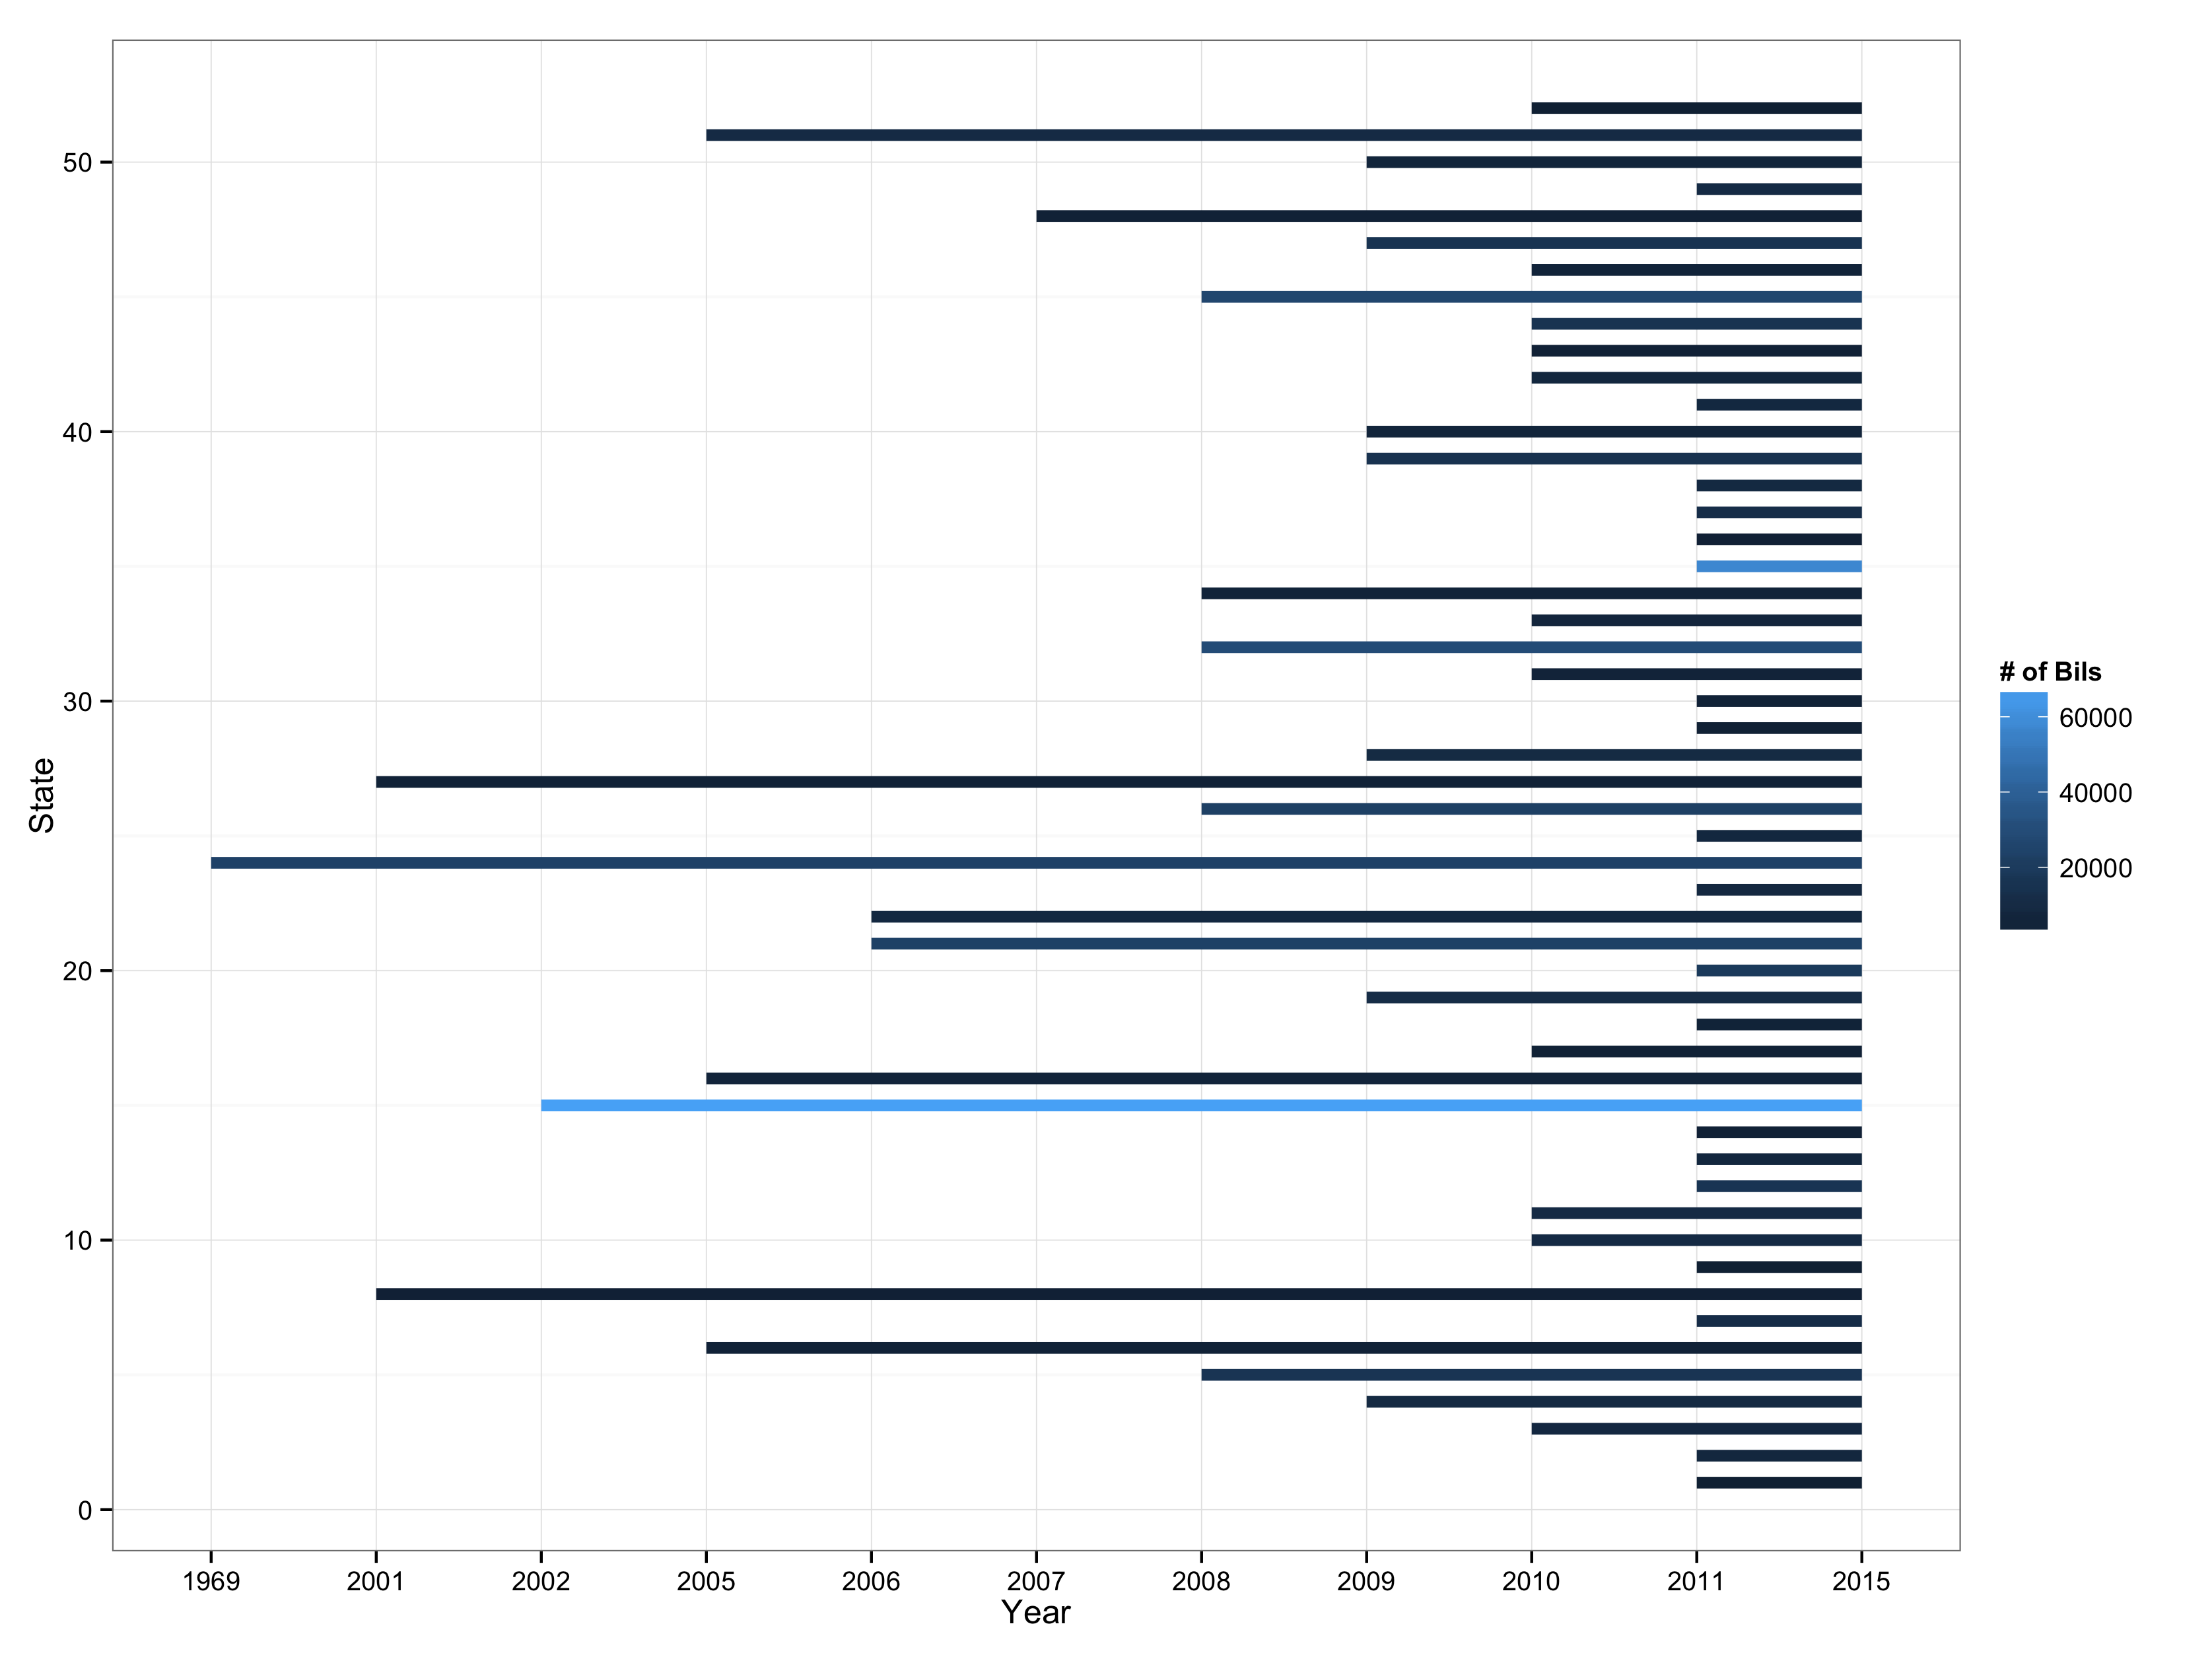
\includegraphics[width=0.9\textwidth]{figures/year_count_by_state.png}
    \caption{Description of the bill database. The horizontal bars display the time range for which bills are available for each state. The color of the bar indicates how many bills are available for this state.}
    \label{fig:bill_desc}
\end{figure}



\textit{Ideological Scores}\\
For the ideological matching, we rely on latent ideology scores measured by \citep{shor2011}. The data set contains scores for 20738 legislators from 50 state legislatures as well as their party affiliation and their time in office. 


\textit{Ground truth - NCSL Tables}\\

To build a ground truth data set, we rely on thematic tables published by the National Council of State Legislatures\footnote{\url{www.ncsl.org}} (NCSL). We collected a sample of these tables with the following procedure:

\begin{singlespacing}

\begin{enumerate}
    \item Collect all urls returned by the web search query: ''site:ncsl.org ''legislation.aspx````\footnote{We used the bing websearch API to collect the urls.}
    \item Sample 50 urls
    \item Select bills that fulfill these three conditions:
        \begin{enumerate}
            \item The website is a NCSL table
            \item The table refers (at least in part) to legislation introduced 2011 or later
            \item The table contains less than 100 individual bills
        \end{enumerate}
    \item Scrape all information from these tables
\end{enumerate}

\end{singlespacing}

Condition a) is necessary, since some of the urls returned by the web query refer to blog entries or to protected websites that require NCSL membership. The rationale behind condition b) is to maximize the number of bills we can match to our database (see Figure \ref{fig:bill_desc}). We additionally constrain the number of bills per table to be below 100, in order to assure, that the topic of the table is not too broad. We chose 100 since this number would correspond roughly to two bills per state (often there is a house and a senate bill in each state for a particular policy).
The web query from step 1 returned 266 urls. From the 50 sampled urls 22 fulfilled the three criteria. From these 22 tables we constructed a dataset of 950 bills, of which we could match 707 to our bill database.


\section{Alignments}

The alignment scores are calculated using the affine version of the local alignment algorithm proposed by \citet{smith1981identification} in order to match genetic sequences. The same algorithm has been used by \citet{wilkerson2015tracing} to trace bills through the legislative process in congress. When considering two bills, the algorithm treats each bill as a sequence of words and tries to find the best alignment between these two sequences. \citet{wilkerson2015tracing} split the bills into sections and search for text reuse across sections. Since this results in about 7 billion possible pairs, first filter out pairs that don't have an exact match of a sequence of at least ten words. We encounter the same problem in our analysis to a greater extent. Assuming each bill consists of ten sections on average, there would be approximately $1.25 * 10^{12}$ possible pairs of sections. 



\section{Analysis}

We use three strategies in order to assess the validity of text reuse as a measure of policy equivalence. First, we apply topic models to the sequences that are identified by the SW algorithm as matching sequences. This provides a rough idea of how many of the alignments are substantial and how much procedural language and not substantively significant language gets picked up by the algorithm. Second, we analyze how well the bill similarity aggregated to the state level corresponds with policy diffusion networks identified in previous research \citep{desmarais2015}. And third, we assess the correlation of the distance of the sponsors of a bill dyad and the dyads alignment scores. If substantive policy content, and importantly, the same ideological direction of the provisions is detected by the alignment algorithm, we will expect a high negative correlation between these two measures.
\subsection{NCSL Tables}

\begin{table}[ht!]
\centering
\caption{My caption}
\label{my-label}
\begin{tabular}{lll}
               & alignment & no alignment \\
not same table & 11        & 232287       \\
same table     & 3083      & 20639       
\end{tabular}
\end{table}

\subsection{Topic Modeling}

We apply statistical topic modeling via Latent Dirichlet Allocation (LDA) \citep{blei2003} to the alignment text with two objectives.\footnote{We use the R package \texttt{mallet} \citep{mallet} for the topic modeling application.} First, we want to see whether the major topical themes that emerge are consistent with policy domains that we would expect to be prominently featured in texts that capture the diffusion of public policy. Second, we want to see whether we can identify topics that correspond to boilerplate/procedural text, which we may want to remove from the alignments to focus the analysis on substantive policy language. In our first cut we use a model with 20 topics. The average alignment is short, with little more than 25\% exceeding 140 characters -- the maximum length of a Tweet. There are 52,735 unique terms in our vocabulary, after removing a standard list of stop words. In Table \ref{tab:top100words} we present the top 100 terms appearing in our corpus. 

\begin{table}[ht]
\rule{\textwidth}{1pt} \\ \vspace{-1cm}
\begin{quotation}
\noindent state person section states act means health public member general commission department law information provided insurance including board subsection legislature benefit court individual property order services care action business time pursuant united date year subject interstate federal compact school insurer corporation required medical chapter provide party entity vehicle amount notice people assembly agreement tax qualified provisions attorney agency limited made service authority child purposes years commissioner education report days policy employer members company code contract employee interest authorized effective statement district purpose ii application period number credit plan include senate income system amended issued reasonable part program director patient requirements
\end{quotation} \vspace{-.5cm}
\rule{\textwidth}{1pt} \vspace{-.2cm}
\caption{Top 100 words, listed left-to-right, in the alignments corpus.}
\label{tab:top100words}
\end{table}

The topic modeling results are presented in Table \ref{tab:topics}. We see that most topics correspond to recognizable policy domains. However, some topics, such as Topic 9, which appears to be a mix of automobile policy and abortion policy, appear to consist of more than one distinct policy domain. As such, we should try running this with more topics. Topic 17 appears to be a boilerplate topic. 

\begin{table}[ht]
\centering
\begin{tabular}{rl}
  \hline
  \hline
6 & benefit corporation public director officer specific interests directors person purpose \\ 
  16 & state order child section support law application employer enforcement court \\ 
  14 & salts isomers food substances substance means preparation product compound mixture \\ 
  3 & court state order person petition section proceeding law appraisal jurisdiction \\ 
  8 & feet distance medical patient marijuana point qualifying south north west \\ 
  20 & information electronic consumer service section insurance notice portable electronics means \\ 
  9 & vehicle motor person means abortion woman medical child dealer death \\ 
  18 & property interest statement section person trust real transfer agreement financing \\ 
  5 & person offense age sexual years criminal court officer sex guilty \\ 
  15 & states united state presidential election official member vote president popular \\ 
  17 & state enacted legislature general assembly people amended section read senate \\ 
  2 & action person section court state civil violation attorney reasonable degree \\ 
  7 & qualified tax section investment revenue entity credit amount fund code \\ 
  19 & health care patient practice medical physician licensed person means services \\ 
  12 & department health state services act public year federal care program \\ 
  4 & appointed members house attorney senate power principal member authority representatives \\ 
  1 & individual employer year years taxable service income employee period january \\ 
  10 & insurance insurer policy commissioner company section coverage contract state plan \\ 
  11 & state commission interstate compact member states rules compacting effective law \\ 
  13 & school student board district education public charter state students county \\ 
   \hline
\end{tabular}
\caption{Results from 200 iterations of LDA with 10 iterations of hyper parameter optimization. Top 10 words in each topic listed for each topic. Topics listed in order of frequency of appearance within documents, beginning in the first row of the table with the most frequent topic.}
\label{tab:topics}
\end{table}

\begin{table}[ht]
\rule{\textwidth}{1pt} \\ \vspace{-1cm}
\begin{quotation}
\noindent state person section states act means health public member general commission department law information provided insurance including board subsection legislature benefit court individual property order services care action business time pursuant united date year subject interstate federal compact school insurer corporation required medical chapter provide party entity vehicle amount notice people assembly agreement tax qualified provisions attorney agency limited made service authority child purposes years commissioner education report days policy employer members company code contract employee interest authorized effective statement district purpose ii application period number credit plan include senate income system amended issued reasonable part program director patient requirements
\end{quotation} \vspace{-.5cm}
\rule{\textwidth}{1pt} \vspace{-.2cm}
\caption{Top 100 words, listed left-to-right, in the alignments corpus.}
\label{tab:top100words}
\end{table}




\subsection{Diffusion networks and Text re-use}

To evaluate whether text re-use corresponds to the transfer of policy, we test whether the presence of a diffusion network tie between two states is a predictor of text reuse. We use the policy diffusion networks inferred in \citet{desmarais2015}. We use [FL FILL IN] to measure the incidence of dyadic text alignment between all state bills covering the time period 200--[??]. For each bill, we first gather the 100 closest bills based on cosine similarity in the term vectors characterizing the bills. We then represent a dyad of bills by the text alignments between them. For each state-pair we calculate the sum of the natural logs of the alignment scores. The ``Diffusion Ties'' variable measures the number of diffusion edges between states in the 2008 diffusion network, as measured by \citet{desmarais2015}. The number of diffusion edges between two states is either 0, 1, or 2. The diffusion network in 2008 is inferred using policy adoptions in the 35 years preceding (and excluding) 2008. As such, we do not risk double-counting bills in the policy adoption and text re-use data. There is one observation in the analysis for each of the 1,225 unique state-pairs. Since this is dyadic data, we use a matrix permutation method, quadratic assignment procedure, to calculate $p$-values \citep{krackhardt1988}. As a robustness check, we run the model with both the identity and log link.\footnote{The $p$-values were calculated using 5,000 random matrix permutations.}

\begin{table}[ht]
\centering
\begin{tabular}{rrrrr}
\hline
& \multicolumn{2}{c}{Identity Link} & \multicolumn{2}{c}{Log Link} \\
  \hline
 & Coefficient & p-value & Coefficient & p-value \\ 
  \hline
Intercept & 21220.1435 & 0.0000 & 9.3643 & 0.0000 \\ 
  Diffusion Ties & 8551.8602 & 0.0352 & 0.3190 & 0.0494 \\ 
   \hline
\end{tabular}
\caption{Predicting number of alignments in legislation across states with diffusion ties. Coefficients calculated with OLS regression. $p$-values based on 5,000 QAP permuations.}
\label{tab:qap.diffusion}
\end{table}

Results of the simple dyadic regression are presented in Table \ref{tab:qap.diffusion}. In both specifications there is a positive relationship between the number of diffusion ties and the number of alignments, and the relationship is statistically significant at the 0.05 level (two-tailed). Furthermore, the magnitudes of the relationships are substantively significant. A shift from the minimum to the maximum number of diffusion ties corresponds to more than a half of a standard deviation increase in the expected number of cross-state alignments. On the log scale, the addition of a diffusion tie corresponds to a 40\% increase in the expected number of cross-state alignments.\footnote{Calculated as $100\times \left[ \exp(0.3288)-1\right] = 38.93$}. 


\subsection{Ideological Distance of Aligned Bills}

%R script for this analysis: '/analysis/ideology.R'

The MALP dataset contains ideal points for about $20,000$ state legislators. The \texttt{openstates} API contains data and identifiers on $12,000$ legislators. Of these we where able to uniquely match about $8,000$ legislators. This allowed us to obtain ideal points for 395,474 ($69\%$) bills and 1,745,336 ($50\%$) pairs of bills. 

In order to assess the validity of text reuse as a measure of substantive policy overlap, we expect the quality of the alignments to be inversely correlated to the distance of the bills sponsors' ideal points. The MALP ideal points are located on a common scale across all states, the distance between sponsors from different states is therefore meaningful. 

In the following sections we present several analyses to assess this correlation. When we are generating the alignments the bills are split up into sections. We generate an alignment score for a bill dyad by summing over all section dyads of the bill dyad.  Table \ref{tab:ideology_regs} displays regression results from a log-linear model regressing the logarithm of the bill dyad alignment score on the ideological distance between the ideal point of the two bills forming the dyad. The ideal point of the bill is derived from the ideal point of the bill sponsor. In cases where several legislators sponsor a bill we use the average of all sponsors' ideal points to obtain a single measure.

The single observations (bill dyads) are not independent, due to the network structure of the data. In order to avoid spurious results, we use the quadratic assignment procedure (QAP), a common tool to control for spurious correlation in social network analysis \citet{krackardt1987qap}. We use 1000 QAP iterations for each model.

% latex table generated in R 3.2.2 by xtable 1.7-4 package
% Mon Dec 21 04:04:01 2015
\begin{table}[ht]
\centering
\begin{tabular}{rrrrr}
  \hline
 & Intercept & Estimate & Std.Dev & p.value \\ 
  \hline
Sum & 4.300 & -0.034 & 0.001 & 0.000 \\ 
  Mean & 3.814 & -0.025 & 0.001 & 0.000 \\ 
  Max & 3.972 & -0.031 & 0.001 & 0.000 \\ 
  No. Alignments & 0.486 & -0.009 & 0.001 & 0.000 \\ 
   \hline
\end{tabular}
\caption{Log-Linear models for alignment and euclidian
distance in ideology. Two tailed p-values are generated from quadratic
assignment procedure with 1000 iterations. Std.Dev is the standard
deviation of the null distribution. The rows correspond to
different methods of aggregating the section alignments to bill
allignments: \textit{Sum}: Sum of alignment scores of all alignments,
\textit{Mean}: Average alignment score accross secion pairs bill dyad,
\textit{Max}: Highest alignment score seciton pairs of bill dyad,
\textit{No. Alignments}: Number of alignments for bill dyad.} 
\label{tab:ideology_regs}
\end{table}


The results in Table \ref{tab:ideology_regs} clearly show that there is a significant correlation between the ideological distance of the bills' sponsors and their text alignment score The null hypothesis of no correlation, the probability for the observed estimate estimated as zero. This is also clear from Figure \ref{fig:qap_dist}, which shows histograms of the permutation distributions of the regression coefficients and the actual estimates as a red line. 

\begin{figure}[ht!]
    \makebox[\textwidth]{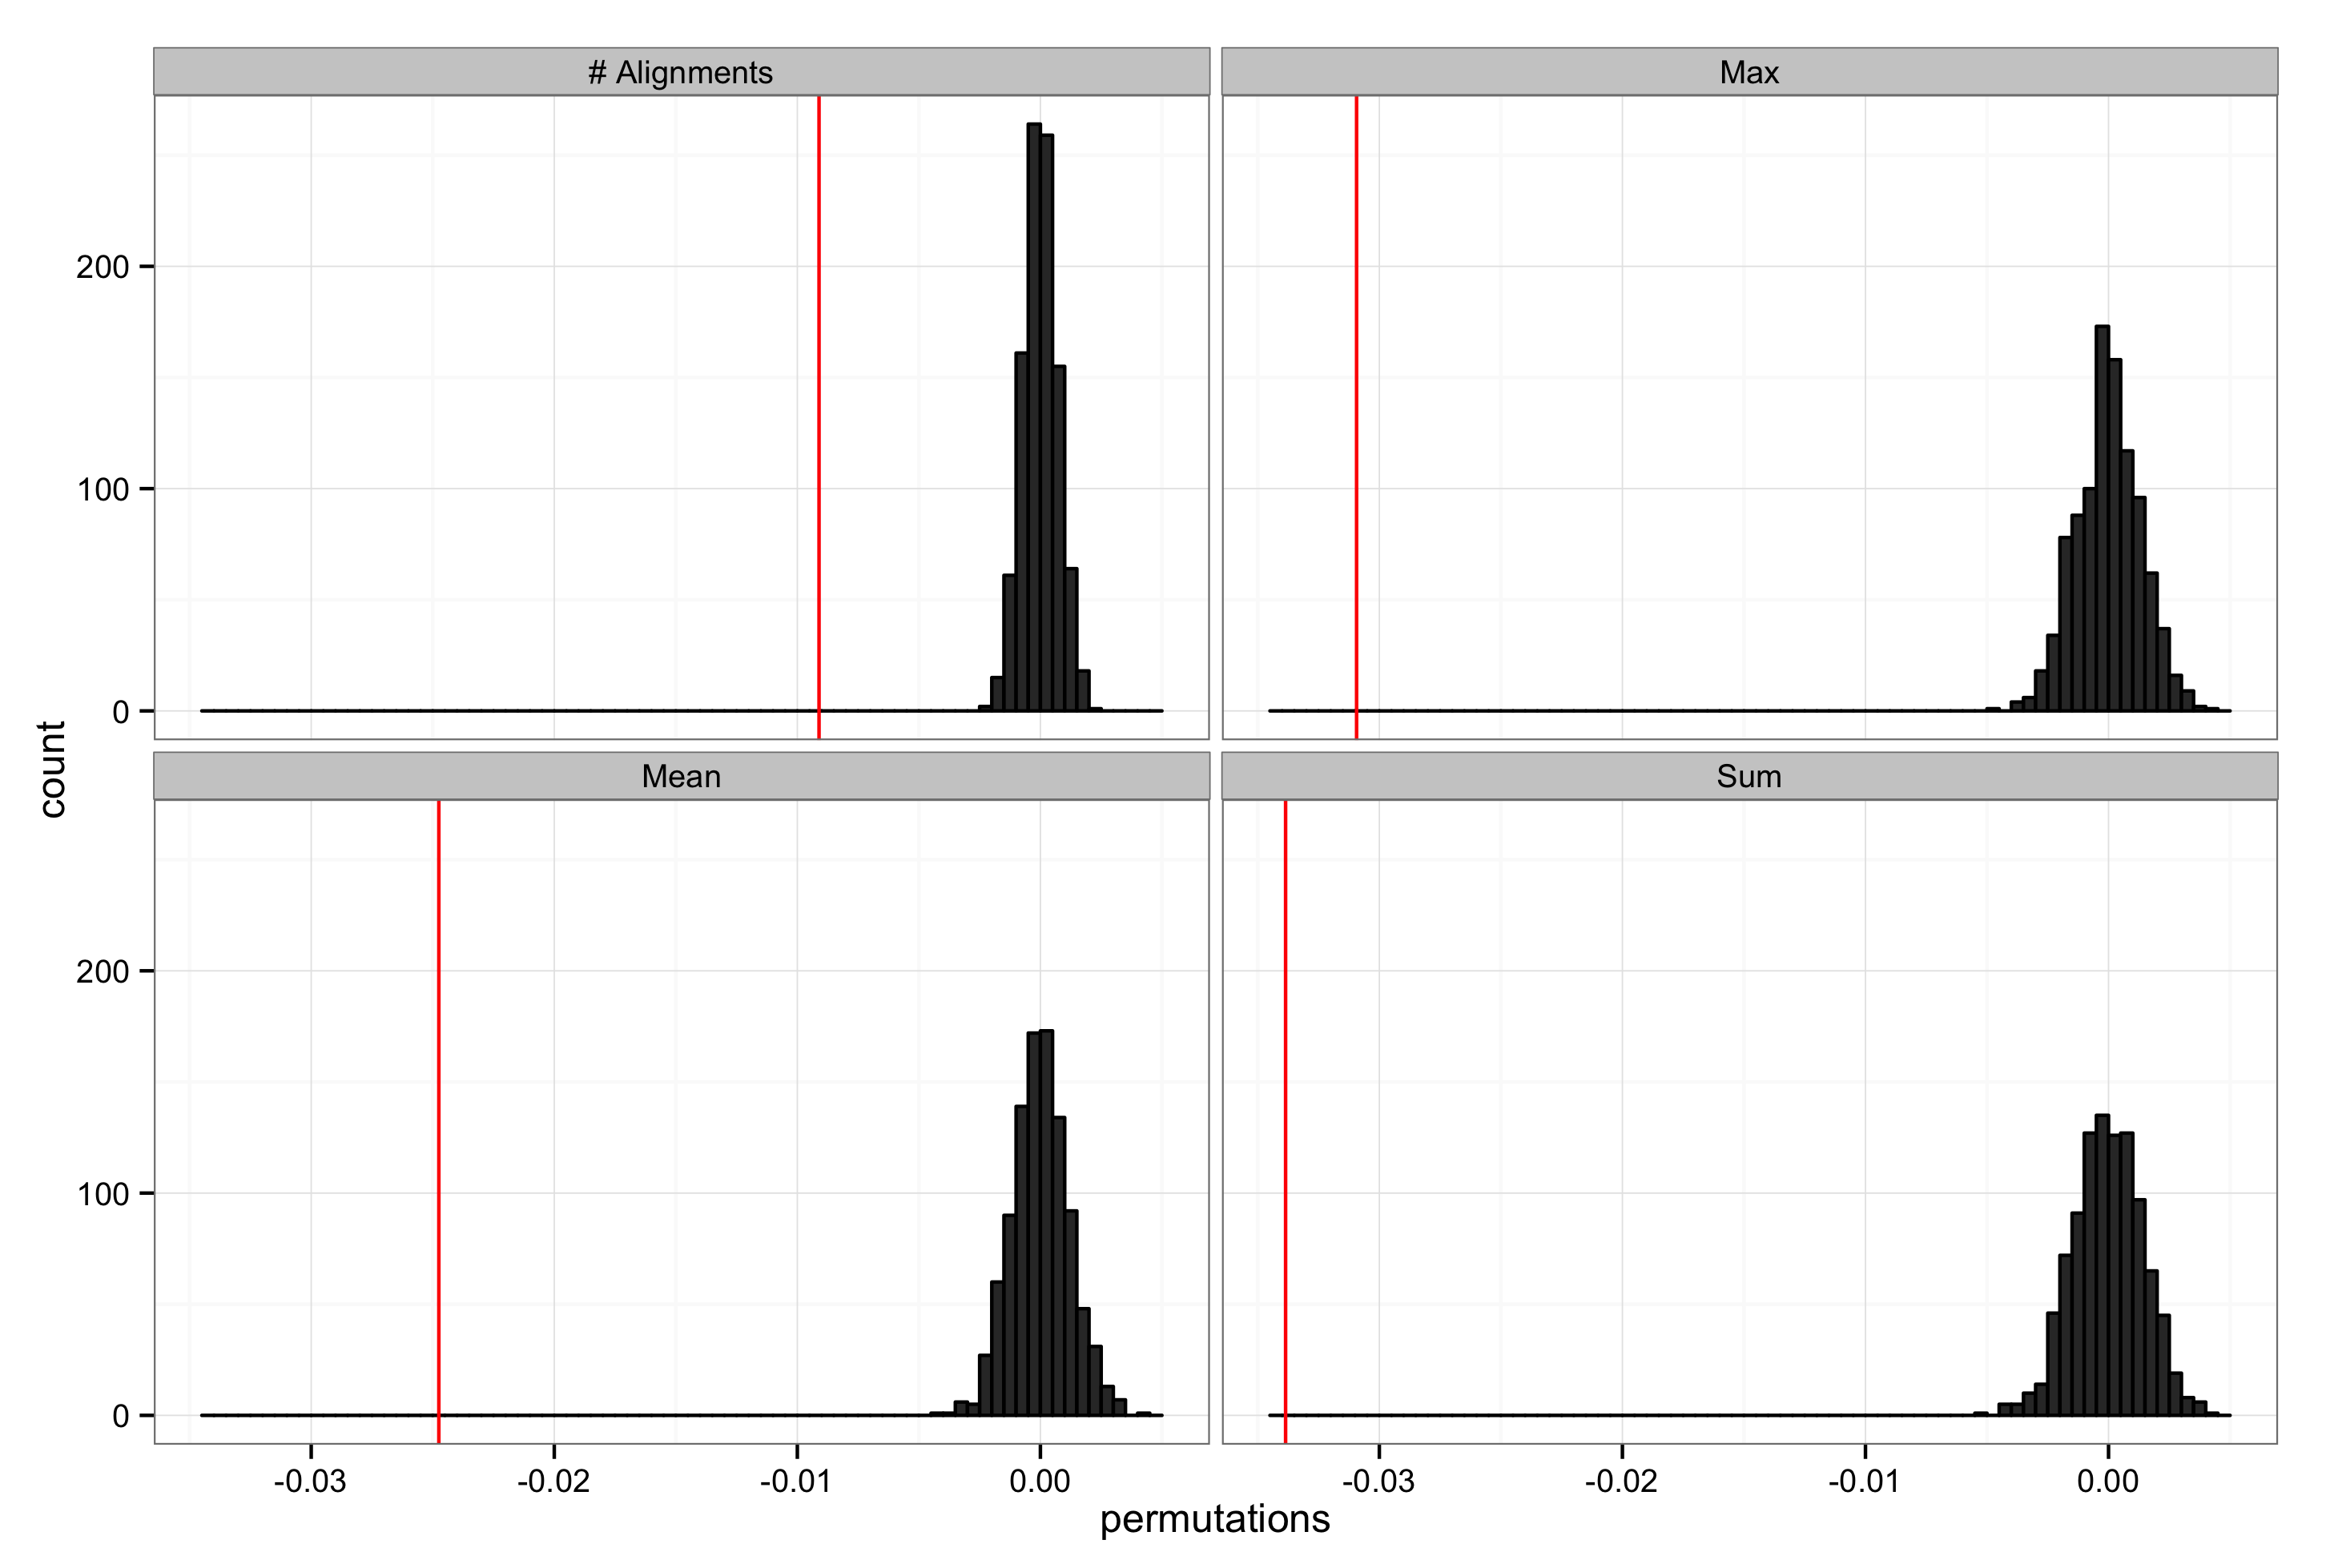
\includegraphics[width=0.9\textwidth]{figures/qap_dist.png}}
\caption{Statistical significance of regression results. The histogram in black shows the distribution of regression coefficients obtained from 1000 qap permutations. The red line displays the estimate obtained from the actual non-permuted network.}
\label{fig:qap_dist}
\end{figure}

To asses the substantive importance of the effect size, Figure \ref{fig:ideo_interpret} displays the estimated decrease in alignment score when increasing the ideological distance of the bills. The vertical lines correspond to the ideological distances between the median democrat and republican, the 0.05 quantile and the 0.95 quantile of the total distribution of ideal points and the minimum and maximum of the total distribution. [FILL IN MORE INTERPRETATION WHEN NEW RESULTS ARE IN] 

\begin{figure}[H]%
\centering
\subfloat[Substantive effects]{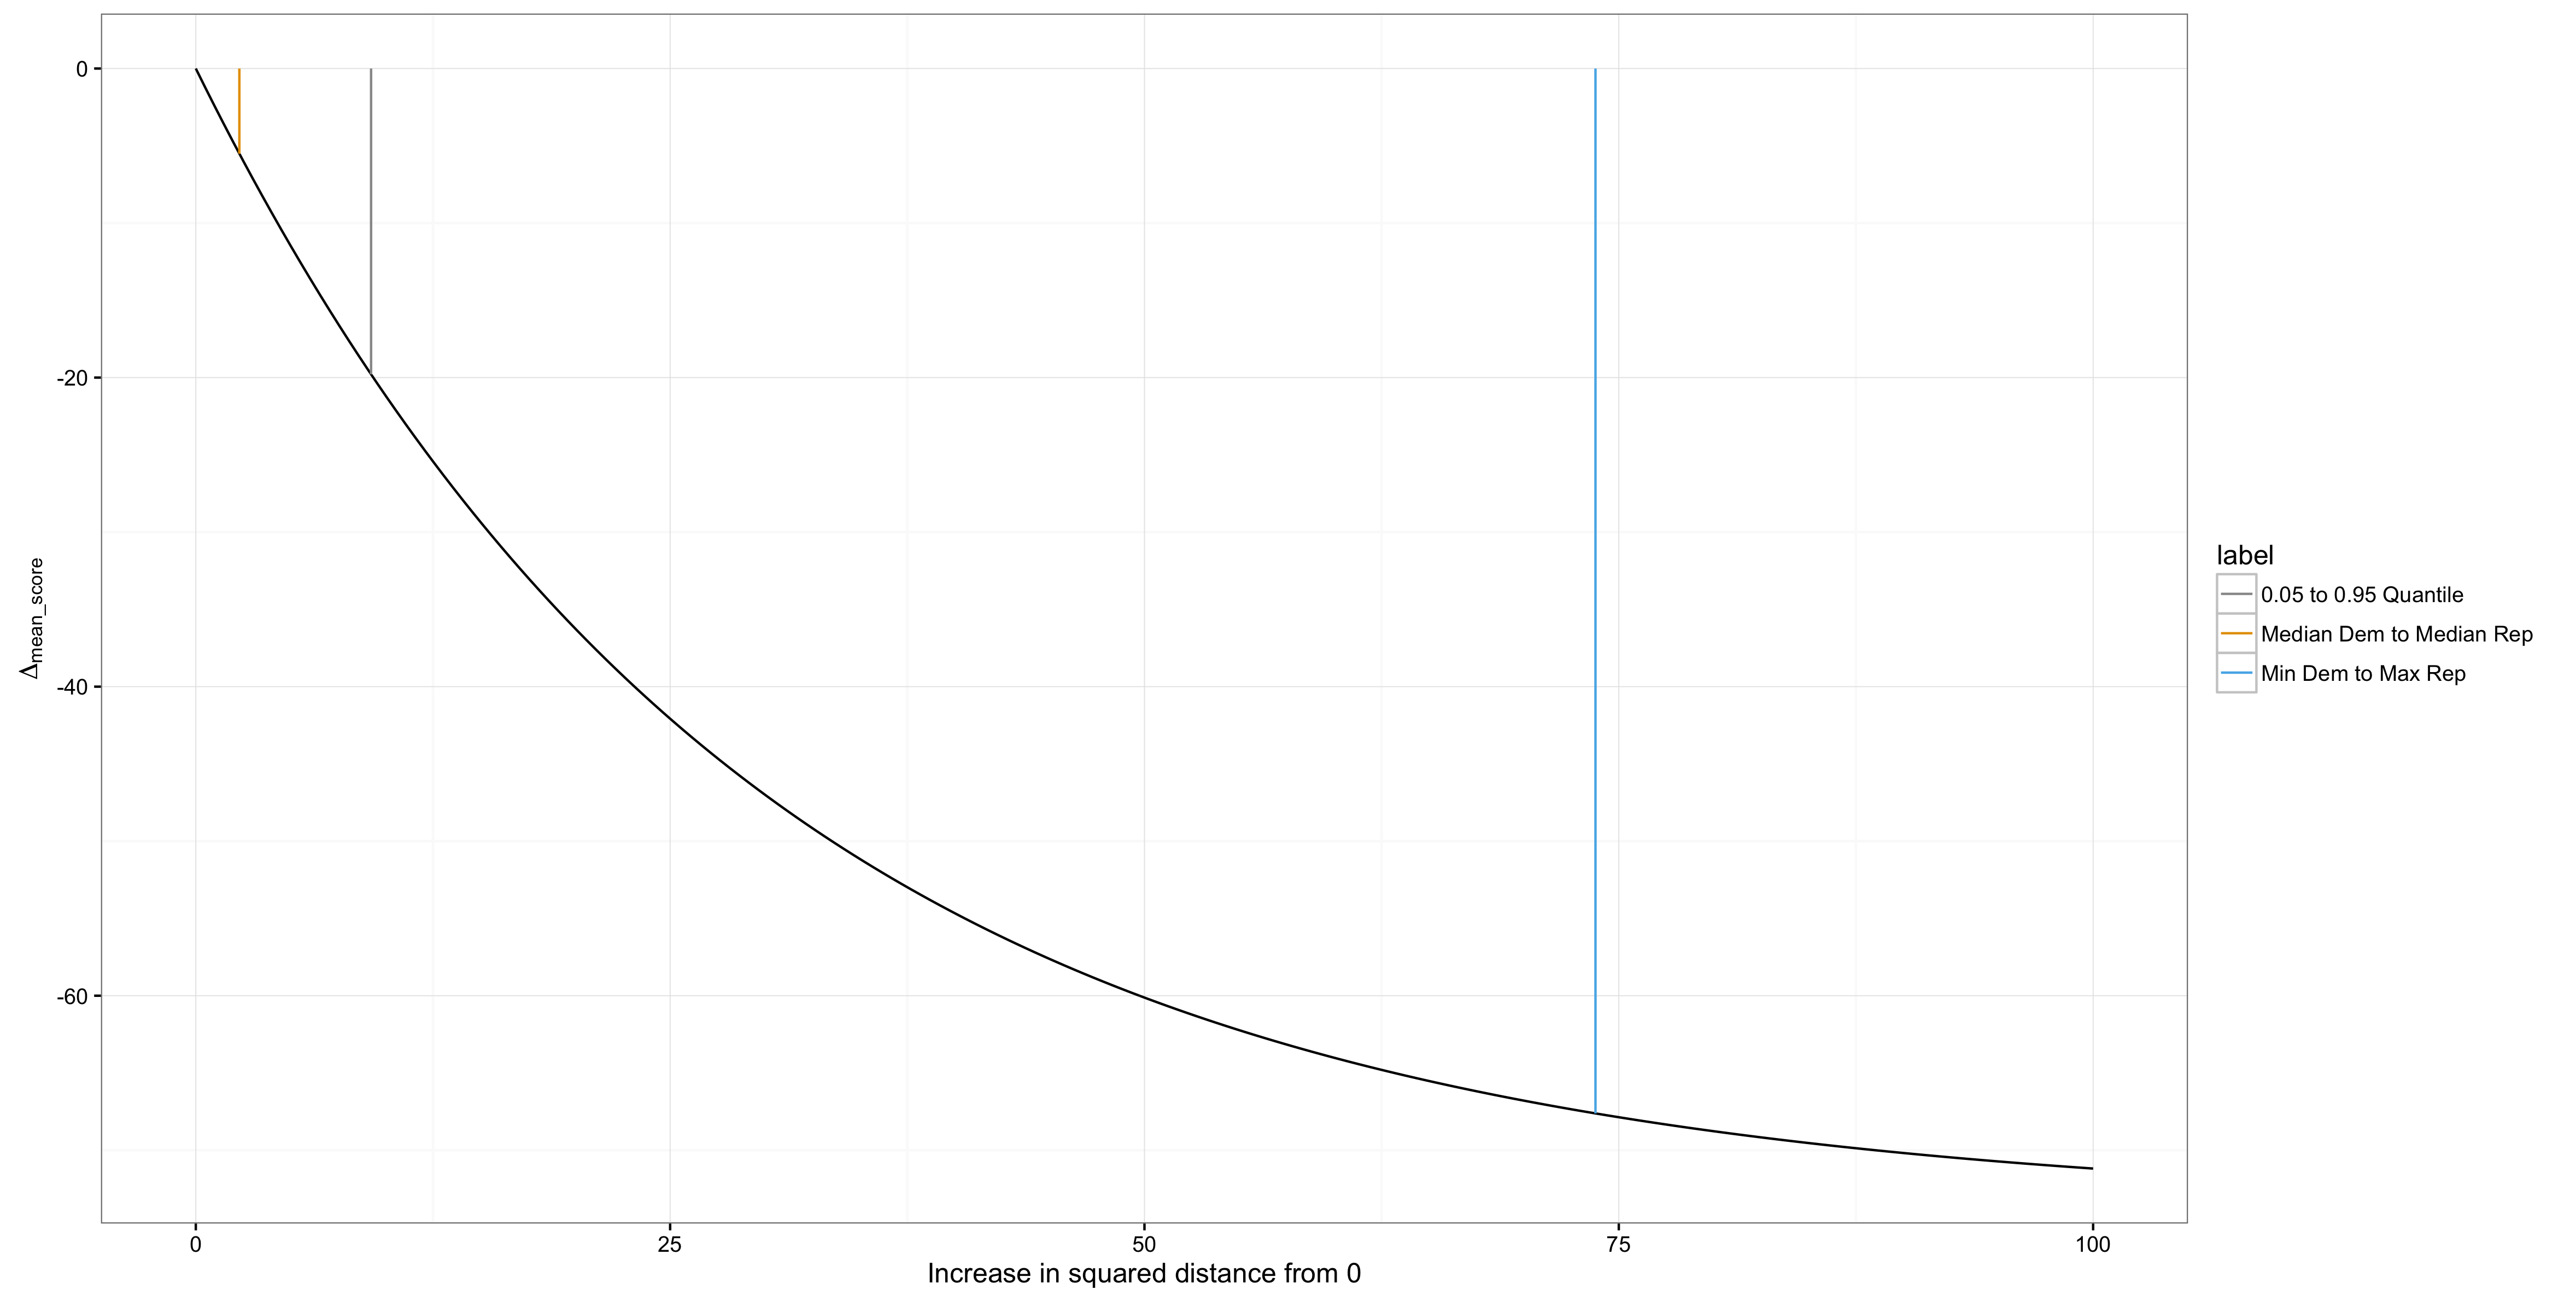
\includegraphics[width=0.5\textwidth]{figures/log_lin_effects.png}}
\subfloat[Distribution of legislator ideal points]{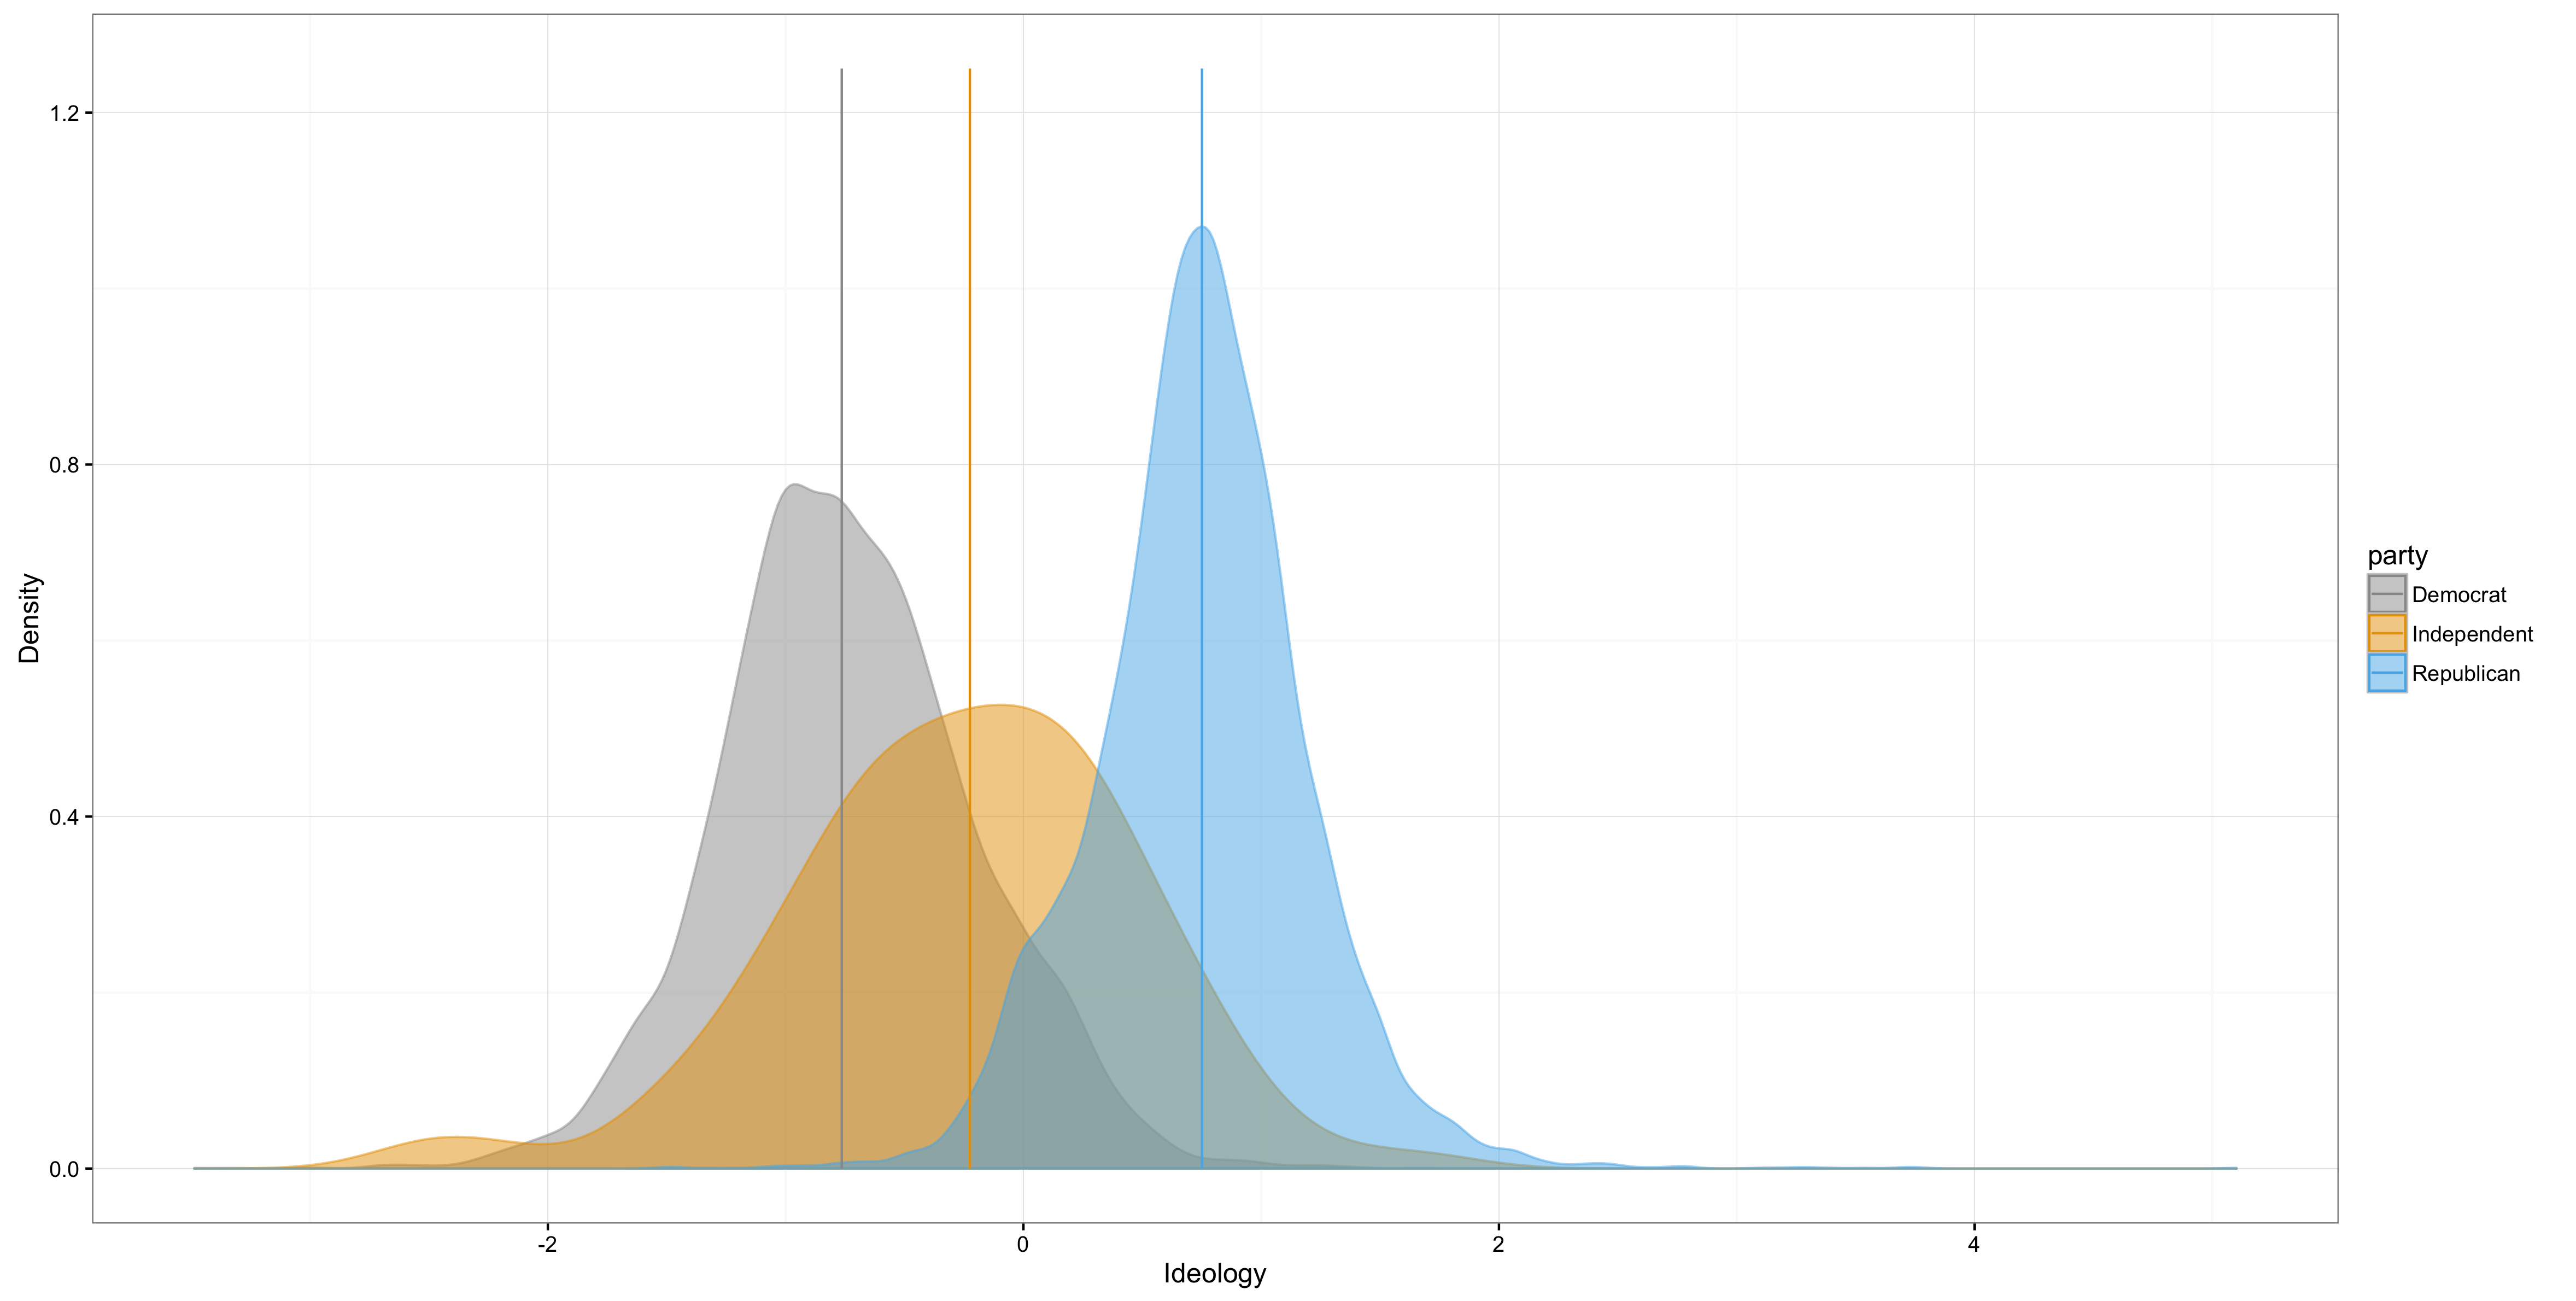
\includegraphics[width=0.5\textwidth]{figures/ideo_distri.png}}
\caption{Substantive interpretation of the effect size of the regression results. The left panel displays the predicted difference in mean alignment score for a change in the ideological distance of the bill. The colored lines connect the distance values to the political landscape. The first line corresponds to the distance between the median democrat and the median republican (across all states), that second line corresponds to the distance between the 0.05 and the 0.95 quantile of the full distribution of legislators' ideal points, and the third line corresponds to the distance from the leftmost to the rightmost legislator. For reference, the left panel displays the kernel density estimate of the distribution of ideal points by party. The vertical lines mark the median ideology for each party. The dependent variable in this illustration is the mean score. Results for different aggregation methods are similar. }
\label{fig:ideo_interpret}
\end{figure}



\clearpage

\bibliographystyle{chicago}
\bibliography{bibliography}


\section{Appendix}

\begin{figure}[ht!]
    \makebox[\textwidth]{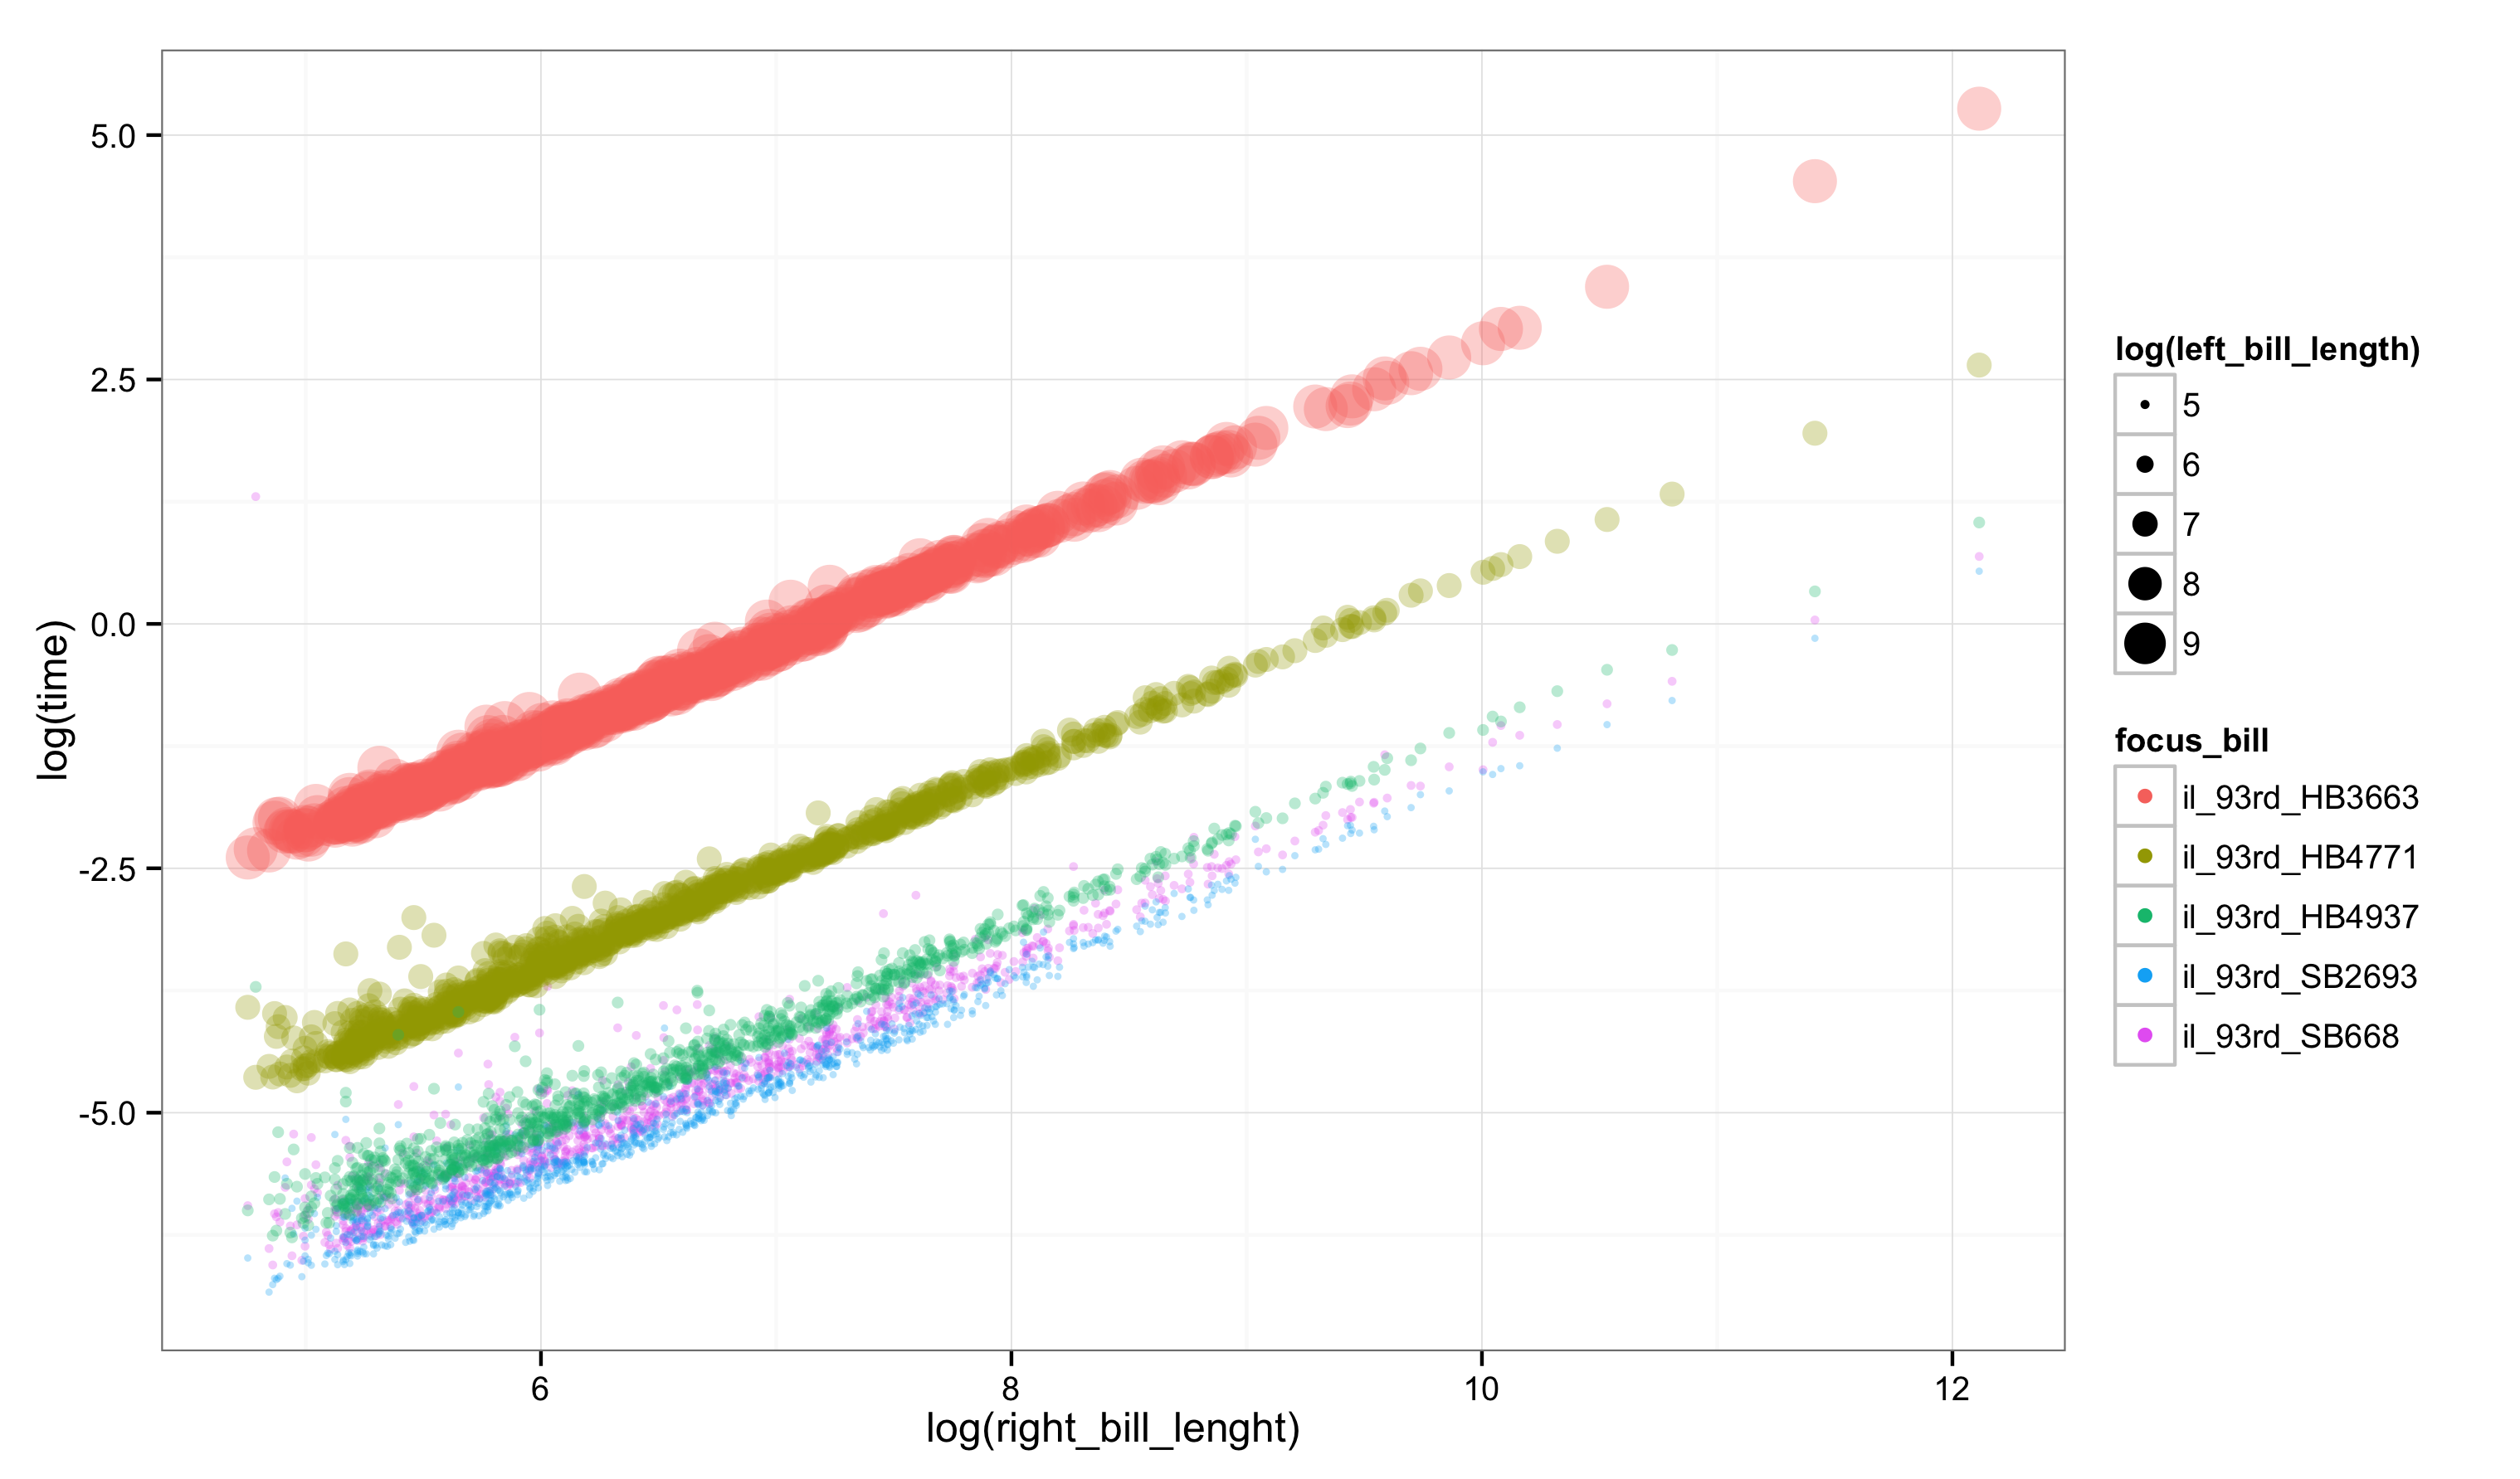
\includegraphics[width=\textwidth]{figures/time_size_selection.png}}
\caption{Computation time for selection of bills. The Colors correspond to five selected bills (focus bill or left bill). For each of the bills, the best alignment with 1000 randomly selected bills (right bills) are calculated. The size of the dots corresponds to the logarithm of the length of the focus bill (in number of words), the x-axis corresponds to the logarithm of the size of the comparison bill and the y-axis corresponds to the logarithm of the computation time (in seconds).}
\label{fig:time_size}
\end{figure}

In order to assess the computational burden the local alignment algorithm poses we test the implementation of the alignment algorithm (Burgess et al. 2015) on a set of 1000 randomly selected bills. In a first pass we calculate the alignments  between all pairs of the full bills (not divided into sections). Figure \ref{fig:time_size} displays the relationship between bill length and computation time. As expected the time increases exponentially with the length of the bills. Figure \ref{fig:time} displays a histogram of the logarithm of the computation time (in seconds). Computation time varies between $0.001s$ and $1,650s$ with $75\%$ of the distribution below $0.1s$ and a median time of $0.03s$.  This shows that an exhaustive comparison of just the full bills (not separated into sections) would take about 100 years on a single machine.

\begin{figure}[ht!]
    \makebox[\textwidth]{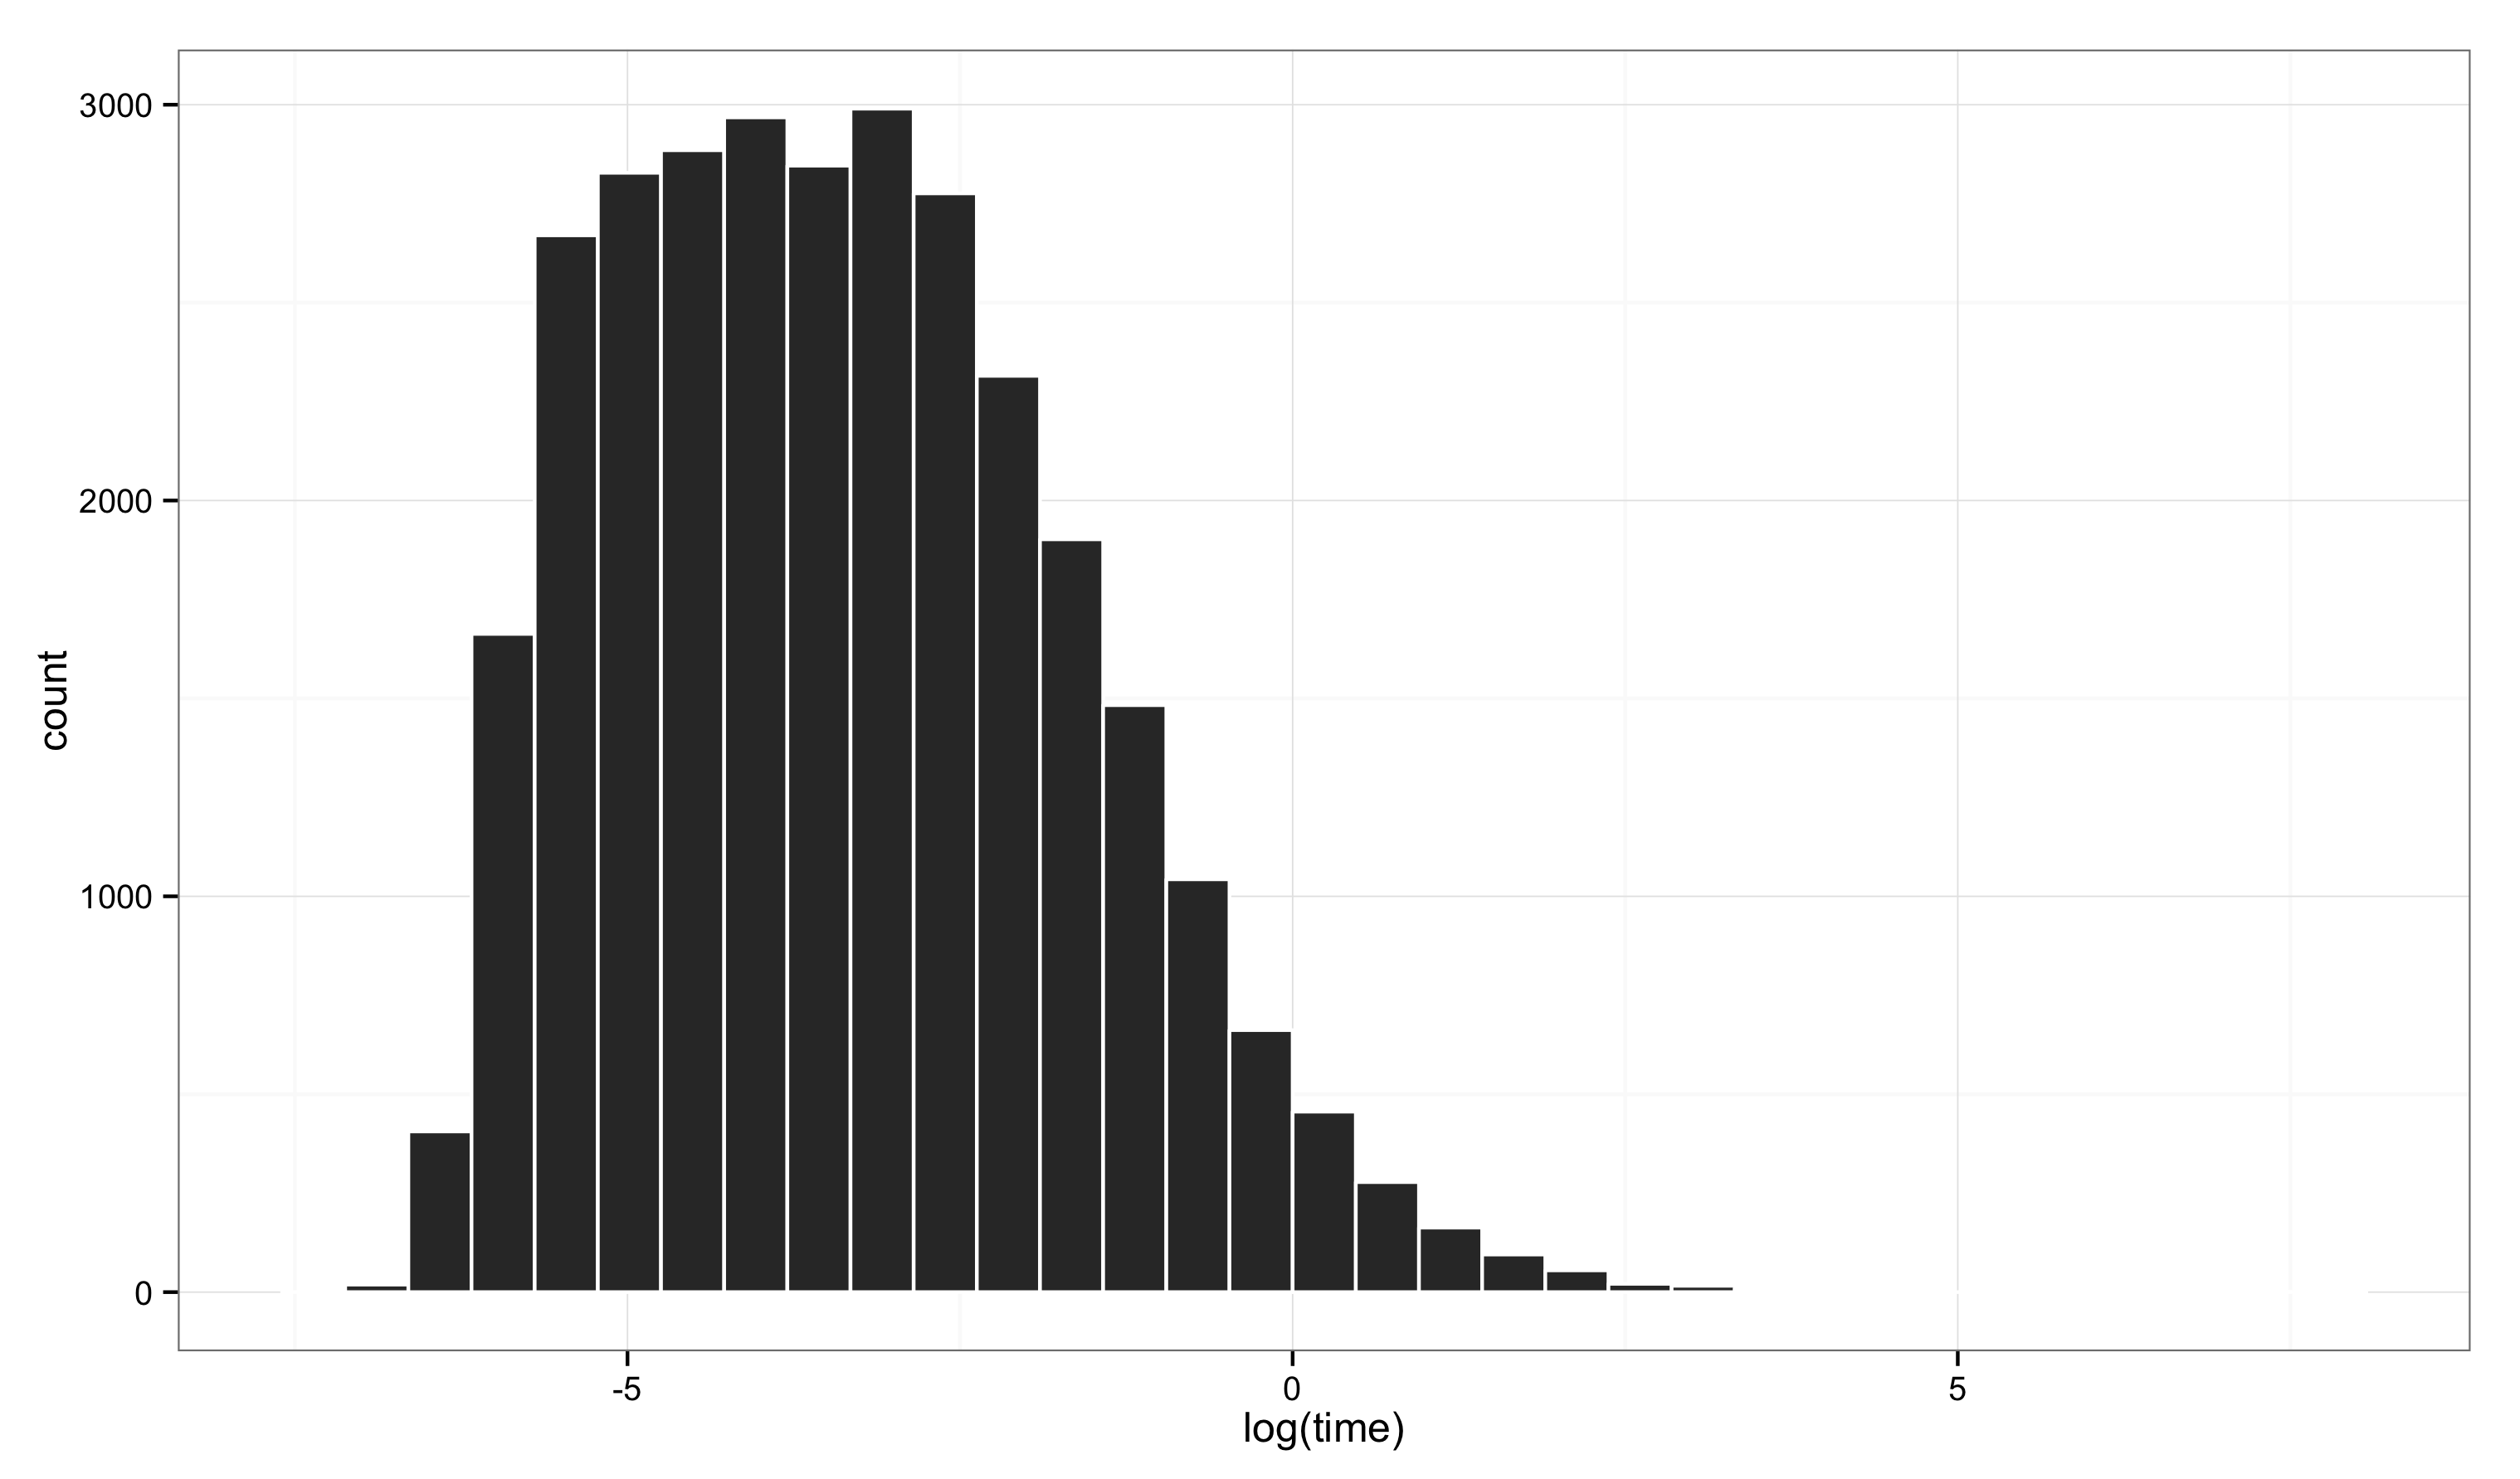
\includegraphics[width=\textwidth]{figures/time.png}}
\caption{Histogram of computation time for all analyzed bills.}
\label{fig:time} 
\end{figure}

Since for this calculation there is no minimum threshold (as in \citet{wilkerson2015tracing} minimum of 5 matching 10-grams). Alignments between almost all bills are found and most of the alignments are procedural language. This is apparent in Figure \ref{fig:state_to_state} which displays the average alignment score for bills from Illinois (left panel) and Washington (right panel) for all other states in the sampled data set (x-axis). Especially for Illinois there is a much higher alignment score for bills from the same state. This shows that a minimum threshold and a classifier for procedural language are necessary.

\begin{figure}[ht!]
    \makebox[\textwidth]{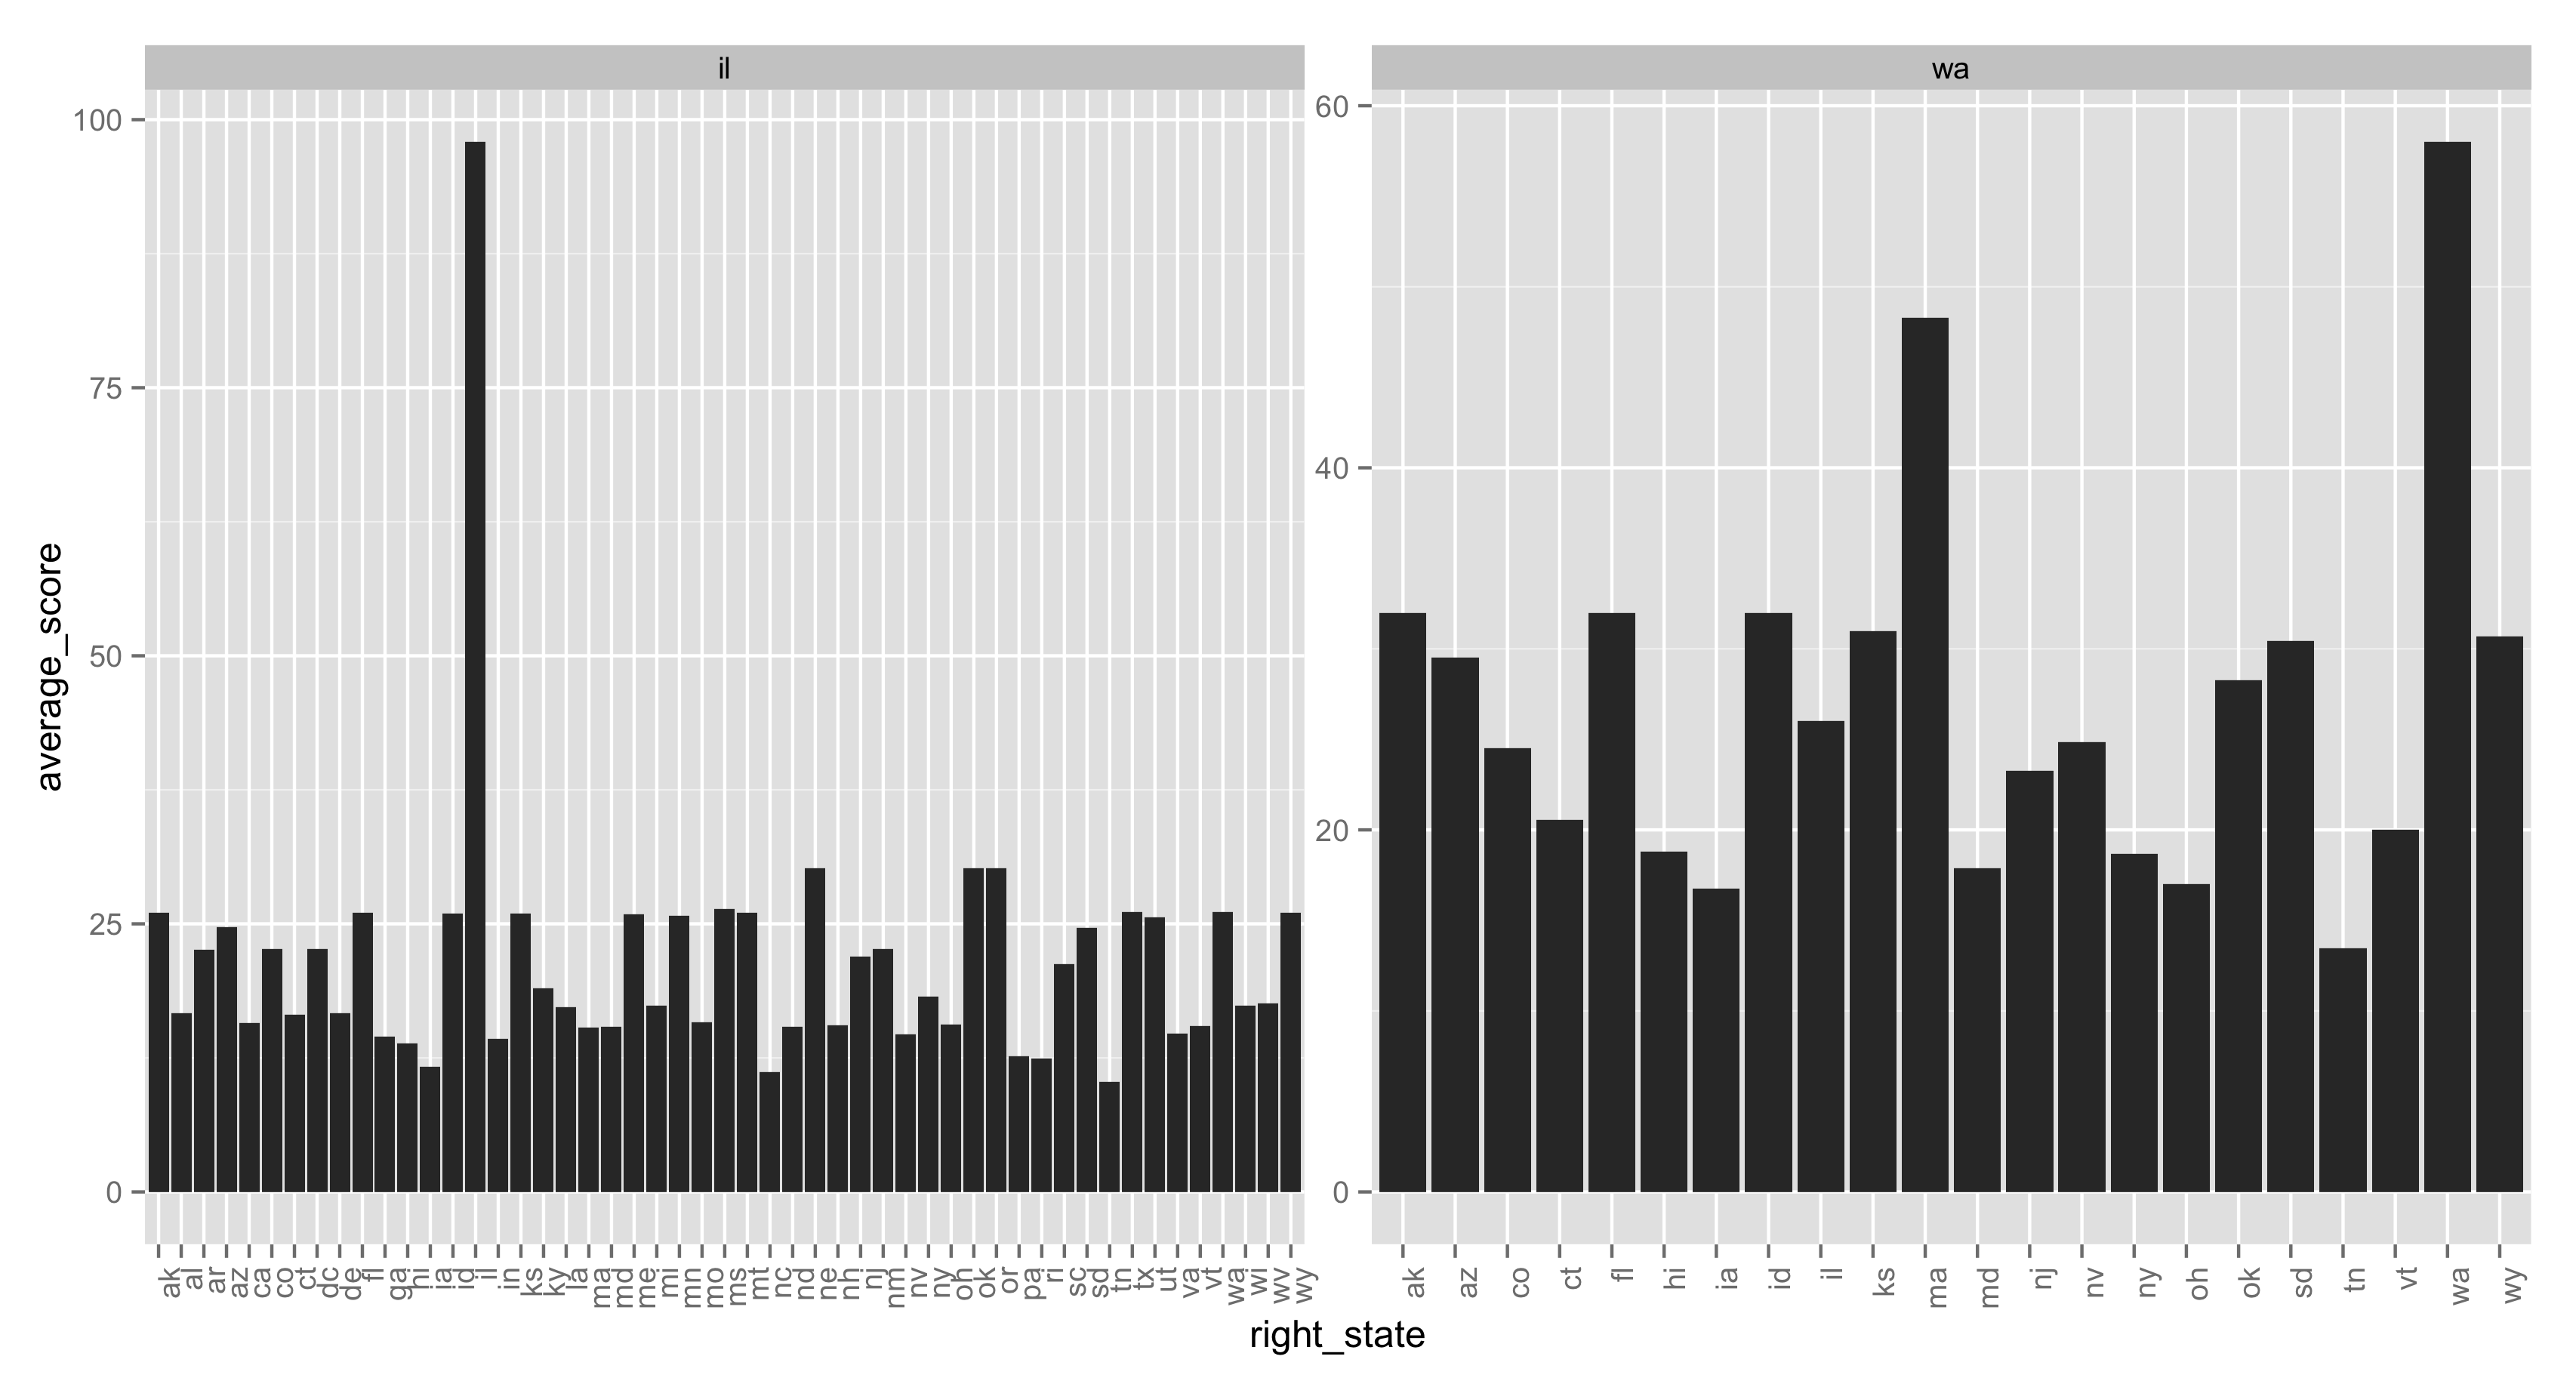
\includegraphics[width=\textwidth]{figures/state_to_state.png}}
\caption{Average alignment scores between states. The left panel corresponds to `left bills' from Illinois, the right panel to bills from Washington. Each bar displays the average score of the best alignment found between bills of the states.}
\label{fig:state_to_state} 
\end{figure}


In order to make the computation more feasible, we rely on a similar strategy as \citet{wilkerson2015tracing}. Our bills are stored in an elastic search database wich provides a variety of search algorithms that are designed to find similar documents. Since seaching the whole database for the full document is very time consuming the following search algorithm is used to first find a pre-selection of similar bills that are then exhaustively checked for text reuse:

\begin{enumerate}
\item All bills are stored in the database in n-grams of size 2-5
\item Select the 25 n-grams with the highest tf-idf score in the query document
\item Calculate a score slightly adapted cosine similarity score between the selected n-gram vector and all full document n-gram vectors in the database\footnote{See \url{https://lucene.apache.org/core/4_9_0/core/org/apache/lucene/search/similarities/TFIDFSimilarity.html} for details on the similarity scoring in Elastic Search}
\end{enumerate}

In order to evaluate how well the pre screening algorithms performs we select 1000 focus bills at random and retrieve the 1000 most similar bills according to the lucene score (described above). We then calculate find the best alignments between the sections of the focus bill and the section of each of the retrieved bills. This procedure generates a dataset of approximately 4 million alignments. 

For a first assessment of the usefulness of the lucene scores to select document that align well, we investigate the relationship of these scores with the alignment scores. Figure \ref{fig:lu_al_scores} displays the lucene scores against the alignment scores for a random sample of 500,000 alignments. The color indicates if the bills from which the alignment was genrated are from the same state, the larger triangles indicate scores for a bill compared to itself. In order to assess which alignments would get selected if thresholding, that is selecting for example the 100 closest bills according to the lucene score, we plotted all alignments for a sample of 9 focus bills. The green points indicate alignments from the 100 bills with the highest lucene scores for the respective focus bill.

\begin{figure}[ht!]
    \makebox[\textwidth]{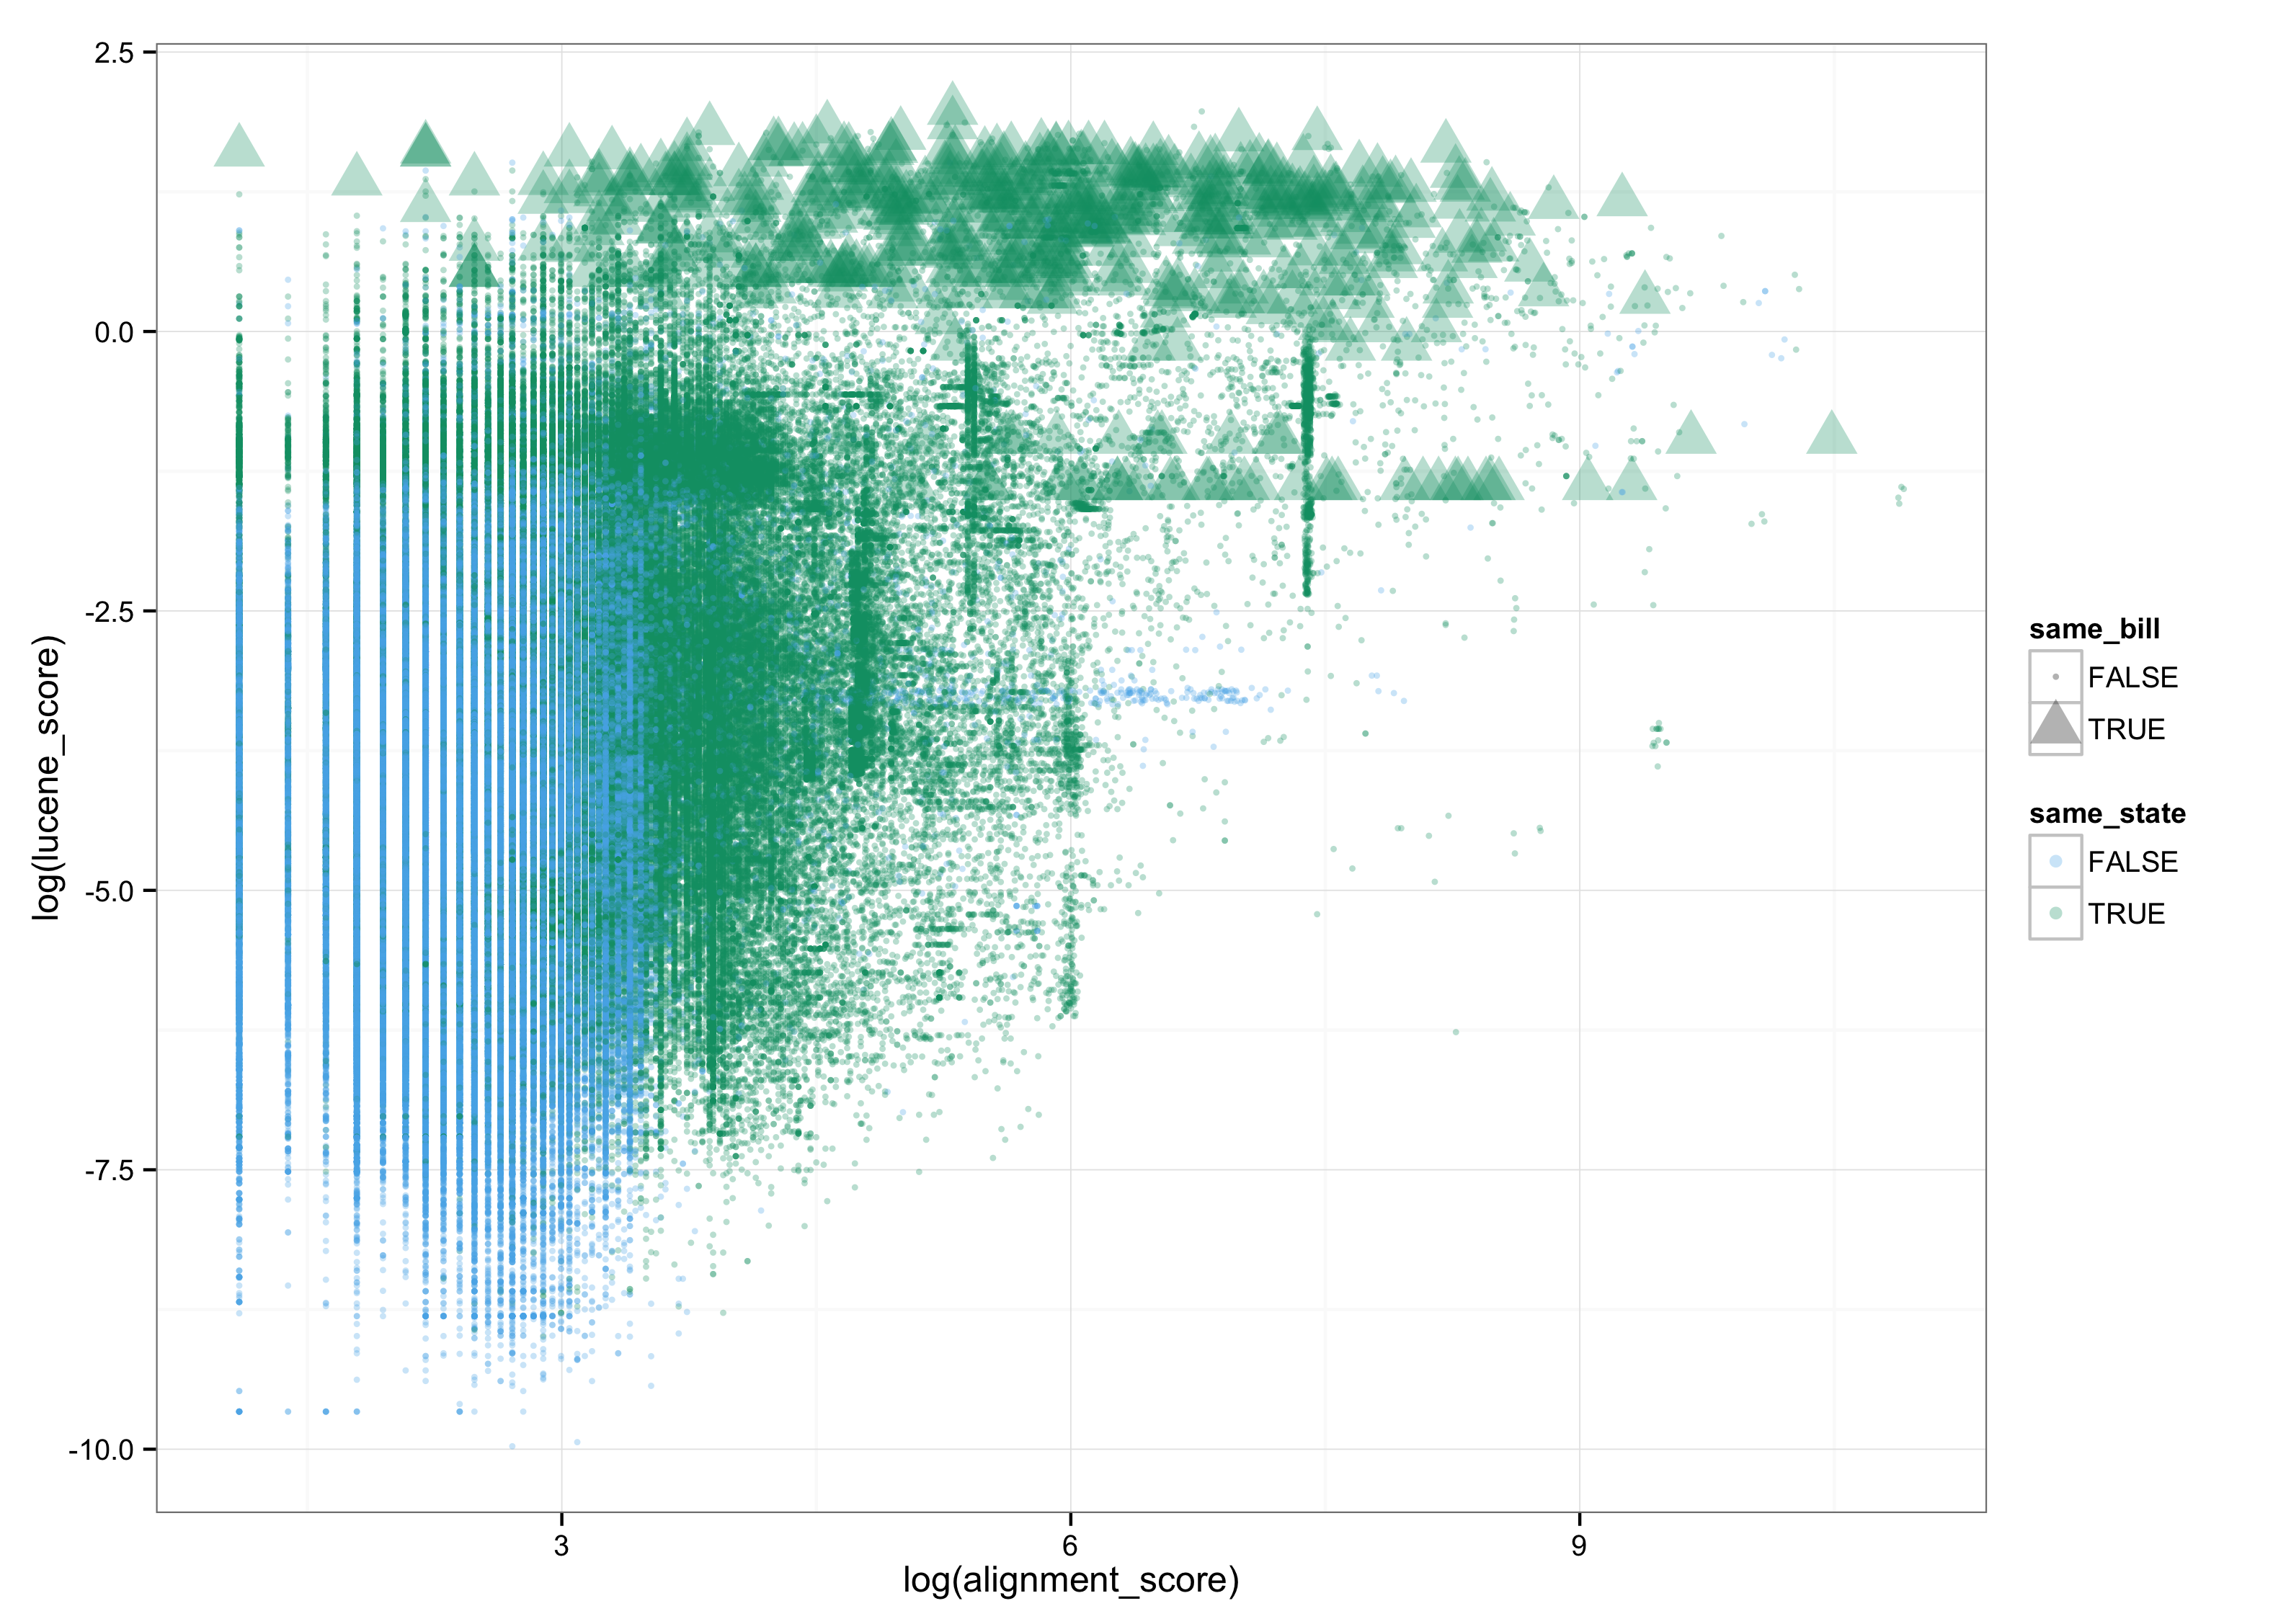
\includegraphics[width=\textwidth]{figures/lu_al_scores.png}}
    \caption{Alignment scores and lucene scores for a sample of 500,000 alignments (sections). The color indicates if the bills of the alignment are from the same state. The larger triangles indicate alignment and lucene scores for sections of bills compared to themselves.}
\label{fig:lu_al_scores} 
\end{figure}

\begin{figure}[ht!]
    \makebox[\textwidth]{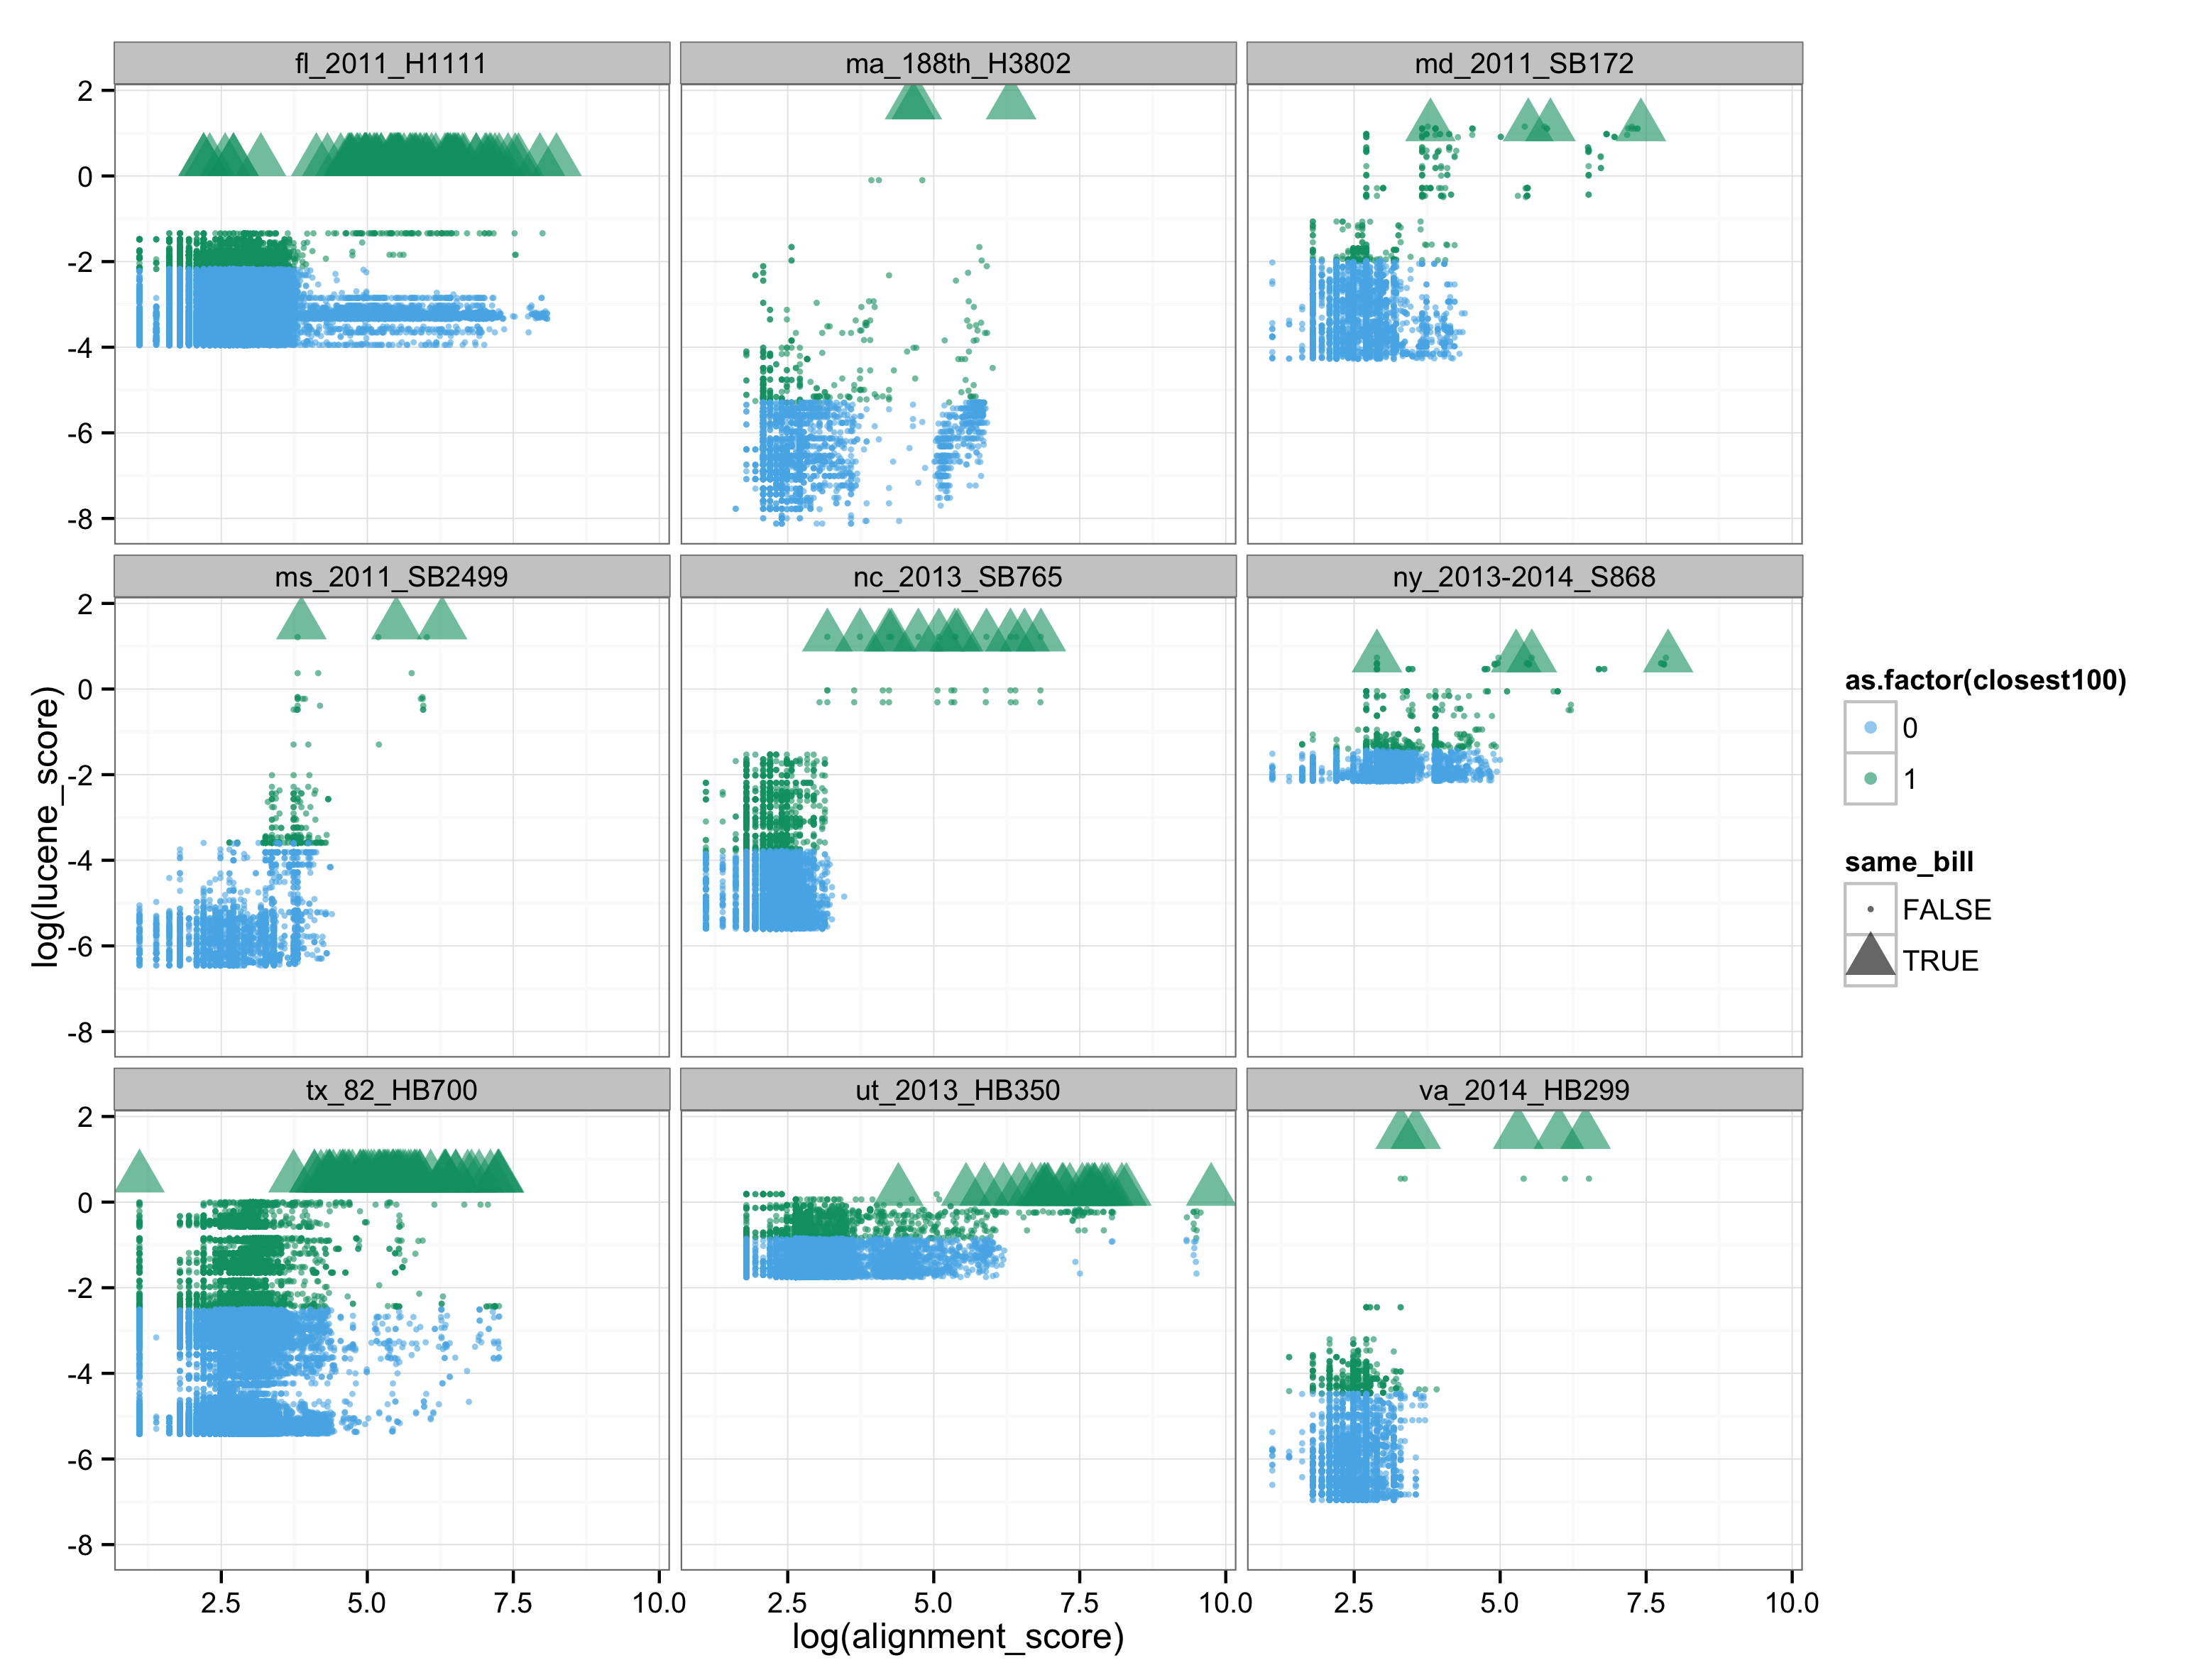
\includegraphics[width=\textwidth]{figures/closest100.png}}
    \caption{Alignment and lucene scores for a sample of nine focus bills (panels). Each point in the plot is an alignment for a section of one comparison bill. The color indicates, if the section comes from a bill that is among the 100 bills with the highest lucene score for the specific focus bill. The large triangles indicate that an alignment is from a comparison of the focus bill with itself.}
\label{fig:closest100} 
\end{figure}



\end{document}
